\chapter{From perception to intensionality}
\label{ch:percint}
\pagestyle{headings}


\section{Perception as type assignment}
\label{sec:perc}

Kim is out for a walk in the park and sees a tree.  She knows that it is a tree
immediately and does not really have to think anything particularly
linguistic, such as ``Aha, that's a tree''.  As a human being with
normal visual perception, Kim is pretty good at recognizing something
as a tree when she sees it, provided that it is a fairly standard
exemplar, and the conditions are right:  for example, there is enough
light and she is
not too far away or too close.  We shall say that Kim's perception of
a certain object, $a$, as a tree involves the ascription of a type
\textit{Tree} to $a$.  In terms of the kind of type theory discussed by
\cite{Martin-Loef1984,NordstromPeterssonSmith1990}, we might say that
Kim has made the \textit{judgement} that $a$ is of type \textit{Tree}
(in symbols $a$ : \textit{Tree}).

% Central to type theory is the notion of judgements that an object $a$
% is of a type $T$ (in symbols $a:T$).  We see this as being
% fundamentally related to perception.

Objects can be of several types.  An object $a$ can be of type
\textit{Tree} but also of type \textit{Oak} (a subtype of
\textit{Tree}, since all objects of type \textit{Oak} are also of type
\textit{Tree}) and \textit{Physical Object} (a supertype of
\textit{Tree}, since all objects of type \textit{Tree} are of type
\textit{Physical Object}).  It might also be of an intuitively more complicated type like
\textit{Objects Perceived by Kim} which is neither a subtype nor a
supertype of \textit{Tree} since not all objects perceived by Kim are
trees and not all trees are perceived by Kim.

There is no perception without some kind of judgement
with respect to types of the perceived object.  When we say that we do
not know what an object is, this normally means that we do not have a
type for the object which is narrow enough for the purposes at hand.
I trip over something in the dark, exclaiming ``What's that?'', but my
painful physical interaction with it through my big toe tells me at
least that
it is a physical object, sufficiently hard and heavy to offer
resistance to my toe.  The act of perceiving an object is perceiving
it \textit{as} something.  You cannot perceive something without
ascribing some type to it, even if it is a very general type such as
\textit{thing} or \textit{entity}.

Recognizing something as a tree may be immediate and not involve
conscious reasoning.  Recognizing a tree as an aspen, an elm or a tree
with Dutch elm disease may involve closer inspection and some conscious
reasoning about the shape of the leaves or the state of the bark.  For
humans the relating of objects to certain types can be the result of a
long chain of reasoning involving a great deal of conscious effort.
But whether the perception is immediate and automatic or the result of
a conscious reasoning process, from a logical point of view it still
seems to involve the ascription of a type to an object.

 

The kind of types we are talking about here correspond to pretty much
any useful way of classifying things and they correspond to what might
be called properties in other theories.  For example, in the classical
approach to formal semantics developed by \cite{Montague1974} and
explicated by \cite{DowtyWallPeters1981} among many others, properties
are regarded not as types but as functions from possible worlds and
times to (the characteristic functions of) sets of entities, that is,
the property \textit{tree} would be a function from possible worlds
and times to the set of all entities which are trees at that world and
time.  Montague has types based on 
a version of Russell's \citeyearpar{Russell1903} simple theory of
types but they were ``abstract'' types like \textit{Entity} and
\textit{Truth Value} and types of functions based on these types
rather than ``contentful'' types like \textit{Tree}.  Type
theory for Montague was a way of providing basic mathematical
structure to the semantic system in a way that would allow the
generation of interpretations of infinitely many natural language
expressions in an orderly fashion that would not get into
problems with logical paradoxes.  The development of the theory of types which
we will undertake here can be regarded as an enrichment of an
``abstract'' type theory like Montague's with ``contentful'' types.
We want to do this in a way that allows the
types to account for content and relate to cognitive processing such
as perception.  We want our types to have psychological relevance and
to correspond to what \cite{Gibson1979} might call
\textit{invariants}, that is, aspects that we can perceive to be the
same when confronted with similar objects or the same object from a
different perspective.  In this respect our types are similar to
notions developed in situation theory and situation semantics
\citep{BarwisePerry1983,Barwise1989}.

Gibson's notion of attunement is adopted by Barwise and Perry.  The
idea is that certain organisms are attuned to certain invariants while
others are not.  Suppose that Kim perceives a cherry tree with flowers
and that a bee alights on one of the flowers.  One assumes that the bee's
experience of the tree is very different from Kim's.  It seems
unlikely that the bee perceives the tree as a tree in the sense that
Kim does and it is not at all obvious that the bee perceives the tree
in its totality as an object.  Different species are attuned to
different types and even within a species different individuals
may vary in the types to which they are attuned.  This means that our
perception is limited by our cognitive apparatus -- not a very
surprising fact, of course, but philosophically very important.  If
perception involves the assignment of types to objects and we are only
able to perceive in terms of those types to which we are attuned, then
as \cite{Kant1781} pointed out we are not actually able to be aware of
\textit{das Ding an sich} (``the thing itself''), that is, we are not
able to be aware of an object independently of the categories (or
types) which are available to us through our cognitive apparatus.
  

\section{Modelling type systems in terms of mathematical objects}

In order to make our theory precise we are going to create
mathematical models of the systems we propose.  This
represents one  of the two main strategies that have been employed in
logic to create rigorous theories.  The other approach is to create a
formal language to describe the objects in the theory and define
rigorous rules of inference which explicate the properties of the
objects and the relations that hold between them.  At a certain level
of abstraction the two approaches are doing the same thing -- in order
to characterize a theory you need to say what objects are involved in
the theory, which important properties they have and what relations
they enter into.  However, the two approaches tend to get associated
with two different logical traditions: the \textit{model theoretic}
and \textit{proof theoretic} traditions.  

The philosophical foundation of type theory (as presented, for
example, by \citealp{Martin-Loef1984}) is normally seen as related to
intuitionism and constructive mathematics.  It is, at bottom,  a proof-theoretic
discipline rather than a model-theoretic one (despite the fact that model
theories have been provided for some type theories).  However, it seems that
many of the ideas in type theory that are important for the analysis
of natural language can be adopted into the classical set theoretic
framework familiar to linguists from the classical model-theoretic canon of formal
semantics starting from \cite{Montague1974}.  We
assume a standard underlying set theory such as ZF
(Zermelo-Fraenkel) with urelements (as formulated for example in \citealp{Suppes1960}).  This is what we take to be the
common or garden working set theory which is familiar from the core
literature on formal semantics deriving from Montague's original work.   

A theory is not very interesting if it does not
make \textit{predictions}, that is, by making certain assumptions you
can infer some conclusions.  This gives you one way to test your
theory:  see what you can conclude from premises that you know or
believe to be true and then test whether the conclusion is actually
true.  If you can show that your theory allows you to predict some
conclusion and its negation, then your theory is
\textit{inconsistent}, which means that it is not useful as a
scientific theory.  One way to discover whether a theory is consistent
or not is to formulate it very carefully and explicitly so that you
can show mathematical properties of the system and any
inconsistencies will appear. 

From the informal discussion of type theory that we have seen so far
it is clear that it should involve two kinds of entity:  the types and
the objects which are of those types.  (Here we use the word
``entity'' not in the sense that Montague did, that is, basic
individuals, but as an informal notion which includes both objects
and types.) This means that we should
characterize a type theory with two domains:
one domain for the objects of the types and another domain for the types to which
these objects belong.  Thus we see types as theoretical entities in
their own right, not, for example, as collections of the objects which
are witnesses for the types.
Diagrammatically we can represent this as in Figure~\ref{fig:basic}
where object $a$ is of type $T_1$.
\begin{figure}[h]
%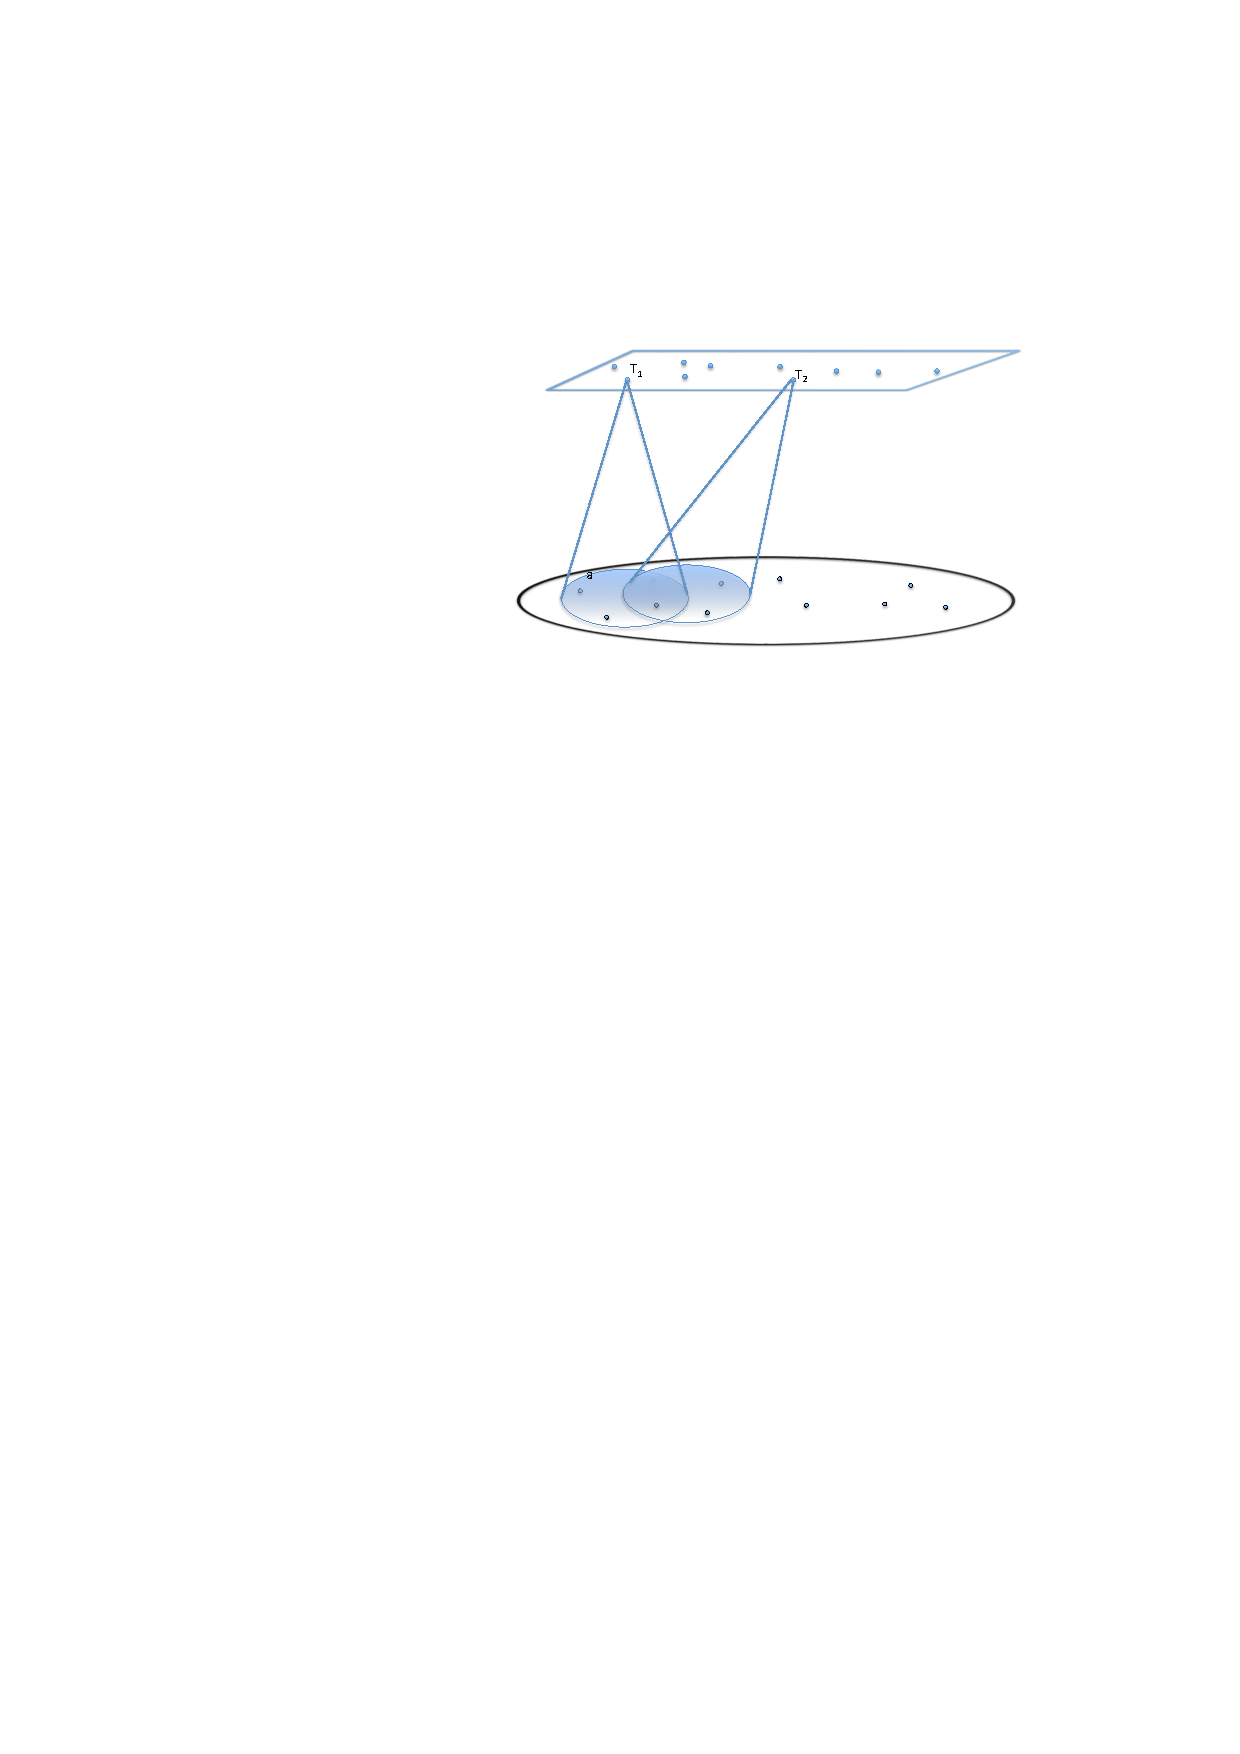
\includegraphics[width=\textwidth]{basic}
\begin{adjustbox}{max width=\textwidth}
\begin{tikzpicture}[
  type/.style={circle, inner sep=0pt, minimum size=6pt, ball color=BTypeCol},
  firsttype/.style={circle, inner sep=0pt, minimum size=6pt, ball color=FirstTypeCol},
  secondtype/.style={circle, inner sep=0pt, minimum size=6pt, ball color=SecondTypeCol},
  objects/.style={circle, inner sep=0pt, minimum size=6pt, ball color=ObjectCol},
  modalobjects/.style={circle, inner sep=0pt, minimum size=6pt, ball color=ModalCol}
  ]

  % basic types:
  \begin{scope}[
    % every node/.append style={yslant=0,xslant=1.75},
    yslant=0,xslant=1.75
    ]
    \filldraw [fill=BTypeCol, draw=BorderCol, thick, fill opacity=0.5] (0,0) rectangle (8,2);

    \foreach \x/\y in {0.5/1.3, 1.4/1.6, 1.8/1.3, 1.9/0.5, 3.3/1.8, 2.6/1.5, 4.4/0.9, 4.7/1, 5.5/0.3, 5.6/1.1, 5.5/1.7, 6.4/1.2, 6.7/1.6} {
      \node [type] at (\x,\y) {};
    }

    \node [coordinate] (btypeleft) at (0,1) {};
    \node [coordinate] (btyperight) at (8,1) {};

    \node [type, label=above:$T_1$] (t1) at (1.3,0.6) {};
    \node [type, label=above:$T_2$] (t2) at (3.1,0.5) {};
  \end{scope}    


  % objects:
  \begin{scope}[
    % every node/.append style={yslant=0,xslant=1.75},
    %yslant=0,xslant=1.75,
    yshift=-100
    ]
    \filldraw [fill=ObjectCol, opacity=0.4, draw=BorderCol, ultra thick] (5,0) ellipse (6 and 1);

    \foreach \a/\b in {5.5/0.7, 6.4/0.2, 6.7/0.6, 7/0, 7.5/0.35, 8/-0.3, 8.1/0.2, 8.7/0, 9/0.2, 10/0.1} {
      \node [objects] at (\a,\b) {};
    }
    % for T1 from BType:
    \node [modalobjects, label=above:$a$] (o1) at (0.3,-0.1) {}; 
    \node [objects] (o2) at (1,0.35) {}; 
    \node [objects] (o3) at (1.6,-0.2) {};
    \node [ellipse, fit=(o1) (o2) (o3), yscale=0.7, draw=BTypeCol, thick, fill=BTypeCol, fill opacity=0.3] (fitA) {};
    \draw [BTypeCol, thick] (t1) -- (fitA.east);
    \draw [BTypeCol, thick] (t1) -- (fitA.west);

    % for T2 from BType:
    \node [objects] (o4) at (2.6,-0.5) {};
    \node [objects] (o5) at (3.1,-0.5) {};
    \node [objects] (o6) at (3.3,-0.1) {};
    \node [ellipse, fit=(o3) (o4) (o5) (o6), yscale=0.7, draw=BTypeCol, thick, fill=BTypeCol, fill opacity=0.2] (fitB) {};
    \draw [BTypeCol, thick] (t2) -- (fitB.east);
    \draw [BTypeCol, thick] (t2) -- (fitB.west);

    % % for T2 from Type1:
     \node [objects] (o7) at (4,0.4) {};
     \node [objects] (o8) at (4.4,0) {}; 
     \node [objects] (o9) at (4.7,0.1) {};
    % \node [ellipse, fit=(o3) (o4) (o5) (o6) (o7) (o8) (o9), yscale=0.6, xscale=0.9, draw=FirstTypeCol, thick, fill=FirstTypeCol, fill opacity=0.2] (fitC) {};

    % % for T2 from Type2:
     \node [objects] (o10) at (5.5,-0.3) {};
     \node [objects] (o11) at (5.6,-0.1) {};
    % \node [ellipse, fit=(o3) (o4) (o5) (o6) (o7) (o8) (o9) (o10) (o11), yscale=0.7, xscale=0.8, draw=SecondTypeCol, thick, fill=SecondTypeCol, fill opacity=0.2] (fitD) {};
  \end{scope}


  % % modal types:
  % \begin{scope}[
  %   % every node/.append style={yslant=0,xslant=1.75},
  %   %yslant=0,xslant=1.75,
  %   yshift=-35, 
  %   xshift=220
  %   ]
  %   \filldraw [fill=ObjectCol, opacity=0.4, draw=BorderCol, ultra thick] (3.5,0) ellipse (4 and 0.75);

  %   \foreach \a/\b in {0.3/-0.1, 1.5/-0.3, 3.9/0.2, 7/0} {
  %     \node [objects] at (\a,\b) {};
  %   }
  %   \node [modalobjects, label=above:$a$] at (0.7,0) {};
  %   \node [objects] (i1) at (5.7,-0.2) {};
  %   \node [objects] (i2) at (6.1,0.3) {};
  %   \node [objects] (i3) at (5,0) {};
  %   \node [ellipse, fit=(i1) (i2) (i3), yscale=0.7, draw=BTypeCol, thick, fill=BTypeCol, fill opacity=0.2] {};

  %   \node [objects] (i4) at (1.6,0.1) {};
  %   \node [objects] (i5) at (2,0.2) {};
  %   \node [modalobjects, label=above:$b$] (i6) at (2.5,-0.3) {};
  %   \node [objects] (i7) at (2.7,0.35) {};
  %   \node [ellipse, fit=(i4) (i5) (i6) (i7), yscale=0.7, xscale=1.1, draw=BTypeCol, thick, fill=BTypeCol, fill opacity=0.2] {};
  % \end{scope}


  % % Type1:
  % \begin{scope}[
  %   % every node/.append style={yslant=0,xslant=1.75},
  %   yslant=0,xslant=1.75,
  %   xshift=-100,
  %   yshift=80
  %   ]
  %   \filldraw [fill=FirstTypeCol, draw=BorderCol, thick, fill opacity=0.3] (0,0) rectangle (8,2);
  %   \node [coordinate] (firsttypeleft) at (0,1) {};
  %   \node [coordinate] (firsttyperight) at (8,1) {};

  %   \foreach \x/\y in {0.45/1.4, 1.4/1.6, 1.9/0.5, 3.3/1.8, 2.6/1.5, 4.7/1, 5.5/0.3, 5.6/1.1,  6.7/1.6} {
  %     \node [firsttype] at (\x,\y) {};
  %   }

  %   \node [firsttype, label=above:$T_1$] (ft1) at (1.8,1.1) {};
  %   \node [firsttype, label=above:$T_2$] (ft2) at (5.8,0.7) {};
  %   \node [firsttype, label=above:$T_3$] (ft3) at (6.4,1.2) {};
  %   \node [firsttype, label=above:{\textbf{Type$^1$}}] (ft) at (4,0.4) {};

  %   \draw [FirstTypeCol, thick] (ft) -- (btypeleft);
  %   \draw [FirstTypeCol, thick] (ft) -- (btyperight);
    
  %   \draw [FirstTypeCol, thick] (ft2) -- (fitC.east);
  %   \draw [FirstTypeCol, thick] (ft2) -- (fitC.west);
  % \end{scope}    


  % % Type2:
  % \begin{scope}[
  %   % every node/.append style={yslant=0,xslant=1.75},
  %   yslant=0,xslant=1.75,
  %   xshift=-200,
  %   yshift=160
  %   ]
  %   \filldraw [fill=SecondTypeCol, draw=BorderCol, thick, fill opacity=0.1] (0,0) rectangle (8,2);
  %   \foreach \x/\y in {1.4/1.6, 1.9/0.5, 3.2/1.5, 4.7/1, 5.4/1.2, 5.8/0.3, 6/0.3,  6.2/1.6} {
  %     \node [secondtype] at (\x,\y) {};
  %   }

  %   \node [secondtype, label=above:$T_1$] (st1) at (1.2,1) {};
  %   \node [secondtype, label=above:$T_2$] (st2) at (4.8,0.7) {};
  %   \node [secondtype, label=above:$T_3$] (st3) at (2.6,1.3) {};
  %   \node [secondtype, label=above:{\textbf{Type$^2$}}] (st) at (3.4,0.5) {};

  %   \draw [SecondTypeCol, thick] (st) -- (firsttypeleft);
  %   \draw [SecondTypeCol, thick] (st) -- (firsttyperight);
    
  %   \draw [SecondTypeCol, thick] (st2) -- (fitD.east);
  %   \draw [SecondTypeCol, thick] (st2) -- (fitD.west);
  % \end{scope}    
\end{tikzpicture}
\end{adjustbox}

\caption{System of basic types}
\label{fig:basic}
\end{figure}

A system of basic types consists of a set of types which are \textit{basic} in
the sense that they are not analyzed as
\textit{complex} entities composed of other entities in the theory.
Each of these types is associated with a set of objects, that is, the
objects which are of the type, the \textit{witnesses} for the type.  Thus if $T$ is a type and $A(T)$ is the
set of witnesses for $T$, then $a$ is of type $T$ (in
symbols, $a:T$) just in case $a\in A(T)$.  We require that any object $a$
which is a witness for a basic type is not itself one of the types in
the system.  A type may be \textit{empty} in the sense that it is
associated with the empty set, that is, there is nothing of that
type. 

Notice that we are starting with the types and associating sets
of objects with them.  This means that while there can be types for
which there are no witnesses, there cannot be objects which do not
belong to a type.  This relates back to our claim in
Section~\ref{sec:perc} that we cannot perceive an object without
assigning a type to it.

Notice also that the sets of objects associated with types may have
members in common.  Thus it is possible for objects to belong to more
than one type.  This is important if we want to have basic types
\textit{Elm}, \textit{Tree} and \textit{Physical Object} and say that
a single object $a$ belongs to all three types as discussed in
Section~\ref{sec:perc}.

An extremely important property of this kind of type system is that
there is nothing which prevents two types from being associated with
exactly the same set of objects.  In standard set theory the notion of
set is \textit{extensional}, that is sets are defined by their
membership.  You cannot have two distinct sets with the same members.
The choice of defining types as entities in their own right rather
than as the sets of their witnesses, means that they can be
\textit{intensional}, that is, you can have more than one type with
the same set of witnesses.  This can be important for the analysis of
natural language words like \textit{groundhog} and \textit{woodchuck}
which (as I have learned from the literature on natural language
semantics) are the same animal. In this case one may wish to say that
you have two different words which correspond to the same type, rather
than two types with the same \textit{extension} (that is, set of
witnesses).  Such an analysis is less appealing in the case of
\textit{unicorn} and \textit{centaur}, both mythical animals
corresponding to types which have an empty extension.  If types were
extensional, there would only be one empty type (just as there is only
one empty set in set theory).  In the kind of possible world semantics
espoused by Montague the distinction between \textit{unicorn} and
\textit{centaur} was made by considering their extension not only in
the actual world (where both are empty) but also in all possible
worlds, since there will be some worlds in which the extensions are
not the same.
However, this kind of possible worlds analysis of intensionality fails
when you have types whose extensions cannot possibly be different.
Consider \textit{round square} and \textit{positive number equal to
  $2-5$}.  The possible worlds analysis cannot distinguish between
these since their extensions are both empty no matter which possible
world you look at.

Finally, notice that there may be different systems of basic types,
possibly with different types and different objects.  One way of
exploiting this would be to associate different systems with different
organisms as discussed in Section~\ref{sec:perc}.  (Below we will see
different uses of this for the analysis of types which model the
cognitive system of a single
agent.) Thus properly we should say that an object $a$ is of type $T$
with respect to a basic systems of types {\bf TYPE$_B$}, in symbols,
$a:_{\mathbf{TYPE_B}}T$.  However,  we will continue
to write $a:T$ in our informal discussion when there is no danger of
confusion. 

The definition of a system of basic types is made precise in
\nexteg{}, which is repeated in
Appendix~\ref{sec:basic}.  

\begin{ex}
A {\it system of basic types\/} is a pair:
\begin{quote}
{\bf TYPE$_B$} = $\langle${\bf Type}, $A$$\rangle$
\end{quote}
where:
\begin{enumerate} 
 
\item \textbf{Type} is a non-empty set 
 
\item $A$ is a function whose domain is \textbf{Type}

\item for any $T\in\textbf{Type}$, $A(T)$ is a set disjoint from
  \textbf{Type}

\item for any $T\in\textbf{Type}$, $a:_{\mathbf{TYPE_B}}T$ iff $a\in A(T)$
 
\end{enumerate}

\label{ex:def-basic-types}
\end{ex} 

Some readers may prefer a slightly less formal characterization which
uses the kind of format normally employed in proof theory.  This may
provide a more easily readable overview of the definitions while
suppressing some of the details which are not necessary for intuitive
understanding.  We will use $\Gamma$, normally used for contexts in
prove theory, that is sequences of judgements to refer to type systems
like those characterized in \preveg{}.  Thus in \nexteg{} $\Gamma$
corresponds to \textbf{TYPE}$_B$.  We will write
$\Gamma\vdash T\in\textbf{Type}$ ``$T\in\textbf{Type}$ follows from
$\Gamma$'' to represent that \textbf{Type} is the set of types in
$\Gamma$  as
specified in \preveg{} and that the type $T$ is a member of this set.
We will similarly write $\Gamma\vdash a\in A(T)$ to indicate that
object $a$ is in the set assigned to $T$ by the function $A$ given by $\Gamma$.
We can then write a rule as in \nexteg{}.
\begin{ex} 
For $\Gamma$ a system of basic types:

\begin{prooftree}
\hypo{\Gamma\vdash T\in \textbf{Type}} \hypo{\Gamma\vdash a\in A(T)}
\infer2{\Gamma\vdash a:T}
\end{prooftree} 
\end{ex} 
We take this to be an inductive definition of the set of consequences.
That is, we are characterizing the smallest set of judgements
$\Gamma\vdash a:T$ which obey the premises.  In this way the inference
rule \preveg{} has the force of a biconditional corresponding to
clause~4 in (\ref{ex:def-basic-types}).   

What counts as an object may vary from agent to agent
(particularly if agents are of different species).  Different agents
have what \cite{Barwise1989} would call different \textit{schemes
  of individuation}.  There appears to be a complex relationship
between the types that an agent is attuned to and the parts of the
world which the agent will perceive as an object.  We model this in
part by allowing different type systems to have different
objects.  In addition we will make extensive use in our systems of a
basic type \textit{Ind} for ``individual'' which corresponds to
Montague's notion of ``entity''.  The type \textit{Ind} might be
thought of as modelling a large part of an agent's scheme of
individuation in Barwise's sense.  However, this clearly still leaves
a great deal to be explained and we do this in the hope that exploring the nature of the type
systems involved will ultimately give us more insight into how
individuation is achieved.


\section{Situation types}
\label{sec:sittypes}

Kim continues her walk in the park.  She sees a boy playing with a dog
and notices that the boy gives the dog a hug.  In perceiving this
event she is aware that two individuals are involved and that there is
a relation holding between them, namely hugging.  She also perceives
that the boy is hugging the dog and not the other way around.  She
sees that a certain action (hugging) is being performed by an agent
(the boy) on a patient (the dog).  This perception seems more complex
than the classification of an individual object as a tree in the sense
that it involves two individual participants and a relation between
them as well as the roles those two individuals play in the relation.
While it is undoubtably more complex than the simple classification of
an object as a tree, we want to say that it is still the assignment of
a type to an object.  The object is now an event and she classifies
the event as a hugging event with the boy as agent and the dog as
patient.  We shall have complex types which can be assigned to such events.

\textit{Complex} types are constructed out of
other entities in the theory.  As we have just seen,
cognitive agents, in addition to being able to assign types to
individual objects like trees, also perceive the world in terms of states and
events where objects have properties and stand in relations to each
other -- what \cite{Davidson1967} called events and
\cite{BarwisePerry1983} called situations.  

\subsection{Types constructed from predicates (ptypes)}
\label{sec:ptypes}
We
introduce types which are constructed from predicates (like `hug') and
objects which are arguments to this predicate like $a$ and $b$.  We
will represent such a constructed type as hug($a$,$b$) and we will
call it a \textit{ptype} to indicate that it is a type whose
main constructor is a predicate.  What would an
object belonging to such a type be?  According to the type-theoretic
approach introduced by Martin-L�f it should be an object which
constitutes a proof that $a$ is hugging $b$.  For Martin-L�f, who was
considering mathematical predicates, such proof objects might be numbers
with certain properties, ordered pairs and so on.  \cite{Ranta1994}
points out that for non-mathematical predicates the objects could be
events as conceived by \cite{Davidson1967,Davidson1980}.  Thus hug($a$,$b$) can be
considered to be an event or a situation type.  In some versions of
situation theory \cite{Barwise1989,SeligmanMoss1997}, objects (called \textit{infons})
constructed from a relation and its arguments was considered to be one
kind of situation type.  Thus one view would be that 
ptypes are playing a similar role in type theory to the role that
infons play in situation theory.

What kind of entity are predicates?  \ignore{The notion is made precise in
Appendix~\ref{app:predicates}.}  One important fact about predicates
is that they come along with an \textit{arity}.  The arity of a
predicate tells you what kind of arguments the predicate takes and
what order they come in. For us the arity of a predicate will be a
sequence of types.  The predicate `hug' as discussed above we can
think of as a two-place predicate both of whose arguments must be of
type \textit{Ind}, that is, an individual.  Thus the arity of `hug'
will be $\langle$\textit{Ind}, \textit{Ind}$\rangle$.  The idea is
that if you combine a predicate with arguments of the appropriate
types in the appropriate order indicated by the arity then you will
have a type.  Thus if $a$ : \textit{Ind} and $b$ : \textit{Ind} then
hug($a$,$b$) will be a type, intuitively the type of situation where
$a$ hugs $b$.  

We will introduce a function \textit{Arity} which is
defined on predicates and which assigns an arity to any predicate.
This function is introduced in a \textit{predicate signature} which in
addition tells you what predicates there are and what we can use to
characterize their arguments (a set of types in the way we will use
this. We define a predicate signature by the definition in \nexteg{}
(repeated in Appendix~\ref{app:predicates}).
\begin{ex} 
A \textit{predicate signature} 
is a triple
\begin{quote}
$\langle$\textbf{Pred}, \textbf{ArgIndices}, \textit{Arity}$\rangle$
\end{quote}
where:
\begin{enumerate} 
 
\item \textbf{Pred} is a set (of predicates)

\item \textbf{ArgIndices} is a set (of indices for predicate
  arguments, normally types)
 
\item \textit{Arity} is a function with domain \textbf{Pred} and range
  included in the set of finite sequences of members of \textbf{ArgIndices}. 
 
\end{enumerate}
\label{ex:pred-sig} 
\end{ex}
A simple example of a predicate signature would be given by \nexteg{}.
\begin{ex} 
\begin{subex} 
 
\item \textbf{Pred} = \{boy, dog, hug\} 
 
\item \textbf{ArgIndices} = \{\textit{Ind}\}

\item \textit{Arity} is defined by:
\begin{quote}
\textit{Arity}(boy) = $\langle\textit{Ind}\rangle$\\
\textit{Arity}(dog) = $\langle\textit{Ind}\rangle$\\
\textit{Arity}(hug) = $\langle\textit{Ind}, \textit{Ind}\rangle$
\end{quote} 
 
\end{subex} 
   
\end{ex} 
   
  

It may be desirable to allow some predicates to combine with more than
one assortment of argument types.  Thus, for example, one might wish
to say that the predicate `believe' can combine with two individuals
just like `hug' (as in \textit{Kim believes Sam}) or with an
individual and a ``proposition'' (as in \textit{Kim believes that Sam
  is telling the truth}).  Similarly the predicate `want' might be
both a two-place predicate for individuals (as in \textit{Kim wants
  the tree}) or a two-place predicate between individuals and
``properties'' (as in \textit{Kim wants to own the tree}).  We shall
have more to say about ``propositions'' and ``properties'' later.  For
now, we just note that we want to allow for the possibilities that
predicates can be \textit{polymorphic} in the sense that there may be
more than one sequence of types which characterize the arguments they
are allowed to combine with.  The sequences need not even be of the
same length (consider \textit{Kim walked} and \textit{Kim walked the
  dog}).  We thus allow for the possibility that these pairs of natural
language examples can be treated using the same polymorphic
predicate.  Another possibility, of course, is to say that the English
verbs can correspond to different (though related) predicates in the
example pairs and not allow this kind of predicate polymorphism in the
type theory. We do not take a stand on this issue but merely note that
both possibilities are available.  If predicates are to be considered
polymorphic then the arity of a predicate can be considered to be a
set of sequences of types.  In \nexteg{} we give a definition of
a polymorphic predicate signature (repeated in Appendix~\ref{app:predicates}).
\begin{ex} 
A \textit{polymorphic predicate signature} 
is a triple 
\begin{quote}
$\langle$\textbf{Pred}, \textbf{ArgIndices}, \textit{Arity}$\rangle$
\end{quote}
where:
\begin{enumerate} 
 
\item \textbf{Pred} is a set (of predicates)

\item \textbf{ArgIndices} is a set (of indices for predicate
  arguments, normally types)
 
\item \textit{Arity} is a function with domain \textbf{Pred} and range
  included in the powerset of the set of finite sequences of members
  of \textbf{ArgIndices}. 
 
\end{enumerate}
\label{ex:poly-pred-sig} 
\end{ex} 
A simple example of a polymorphic predicate signature is given in
\nexteg{}.
\begin{ex} 
\begin{subex} 
 
\item \textbf{Pred} = \{boy, dog, hug, walk\} 
 
\item \textbf{ArgIndices} = \{\textit{Ind}\}

\item \textit{Arity} is defined by:
\begin{quote}
\textit{Arity}(boy) = $\{\langle\textit{Ind}\rangle\}$\\
\textit{Arity}(dog) = $\{\langle\textit{Ind}\rangle\}$\\
\textit{Arity}(hug) = $\{\langle\textit{Ind}, \textit{Ind}\rangle\}$\\
\textit{Arity}(walk) = $\{\langle\textit{Ind}\rangle, \langle\textit{Ind}, \textit{Ind}\rangle\}$
\end{quote} 
 
\end{subex} 
   
\end{ex}   

An alternative to our characterization of predicates is to consider them as functions from sequences of objects
matching their arity to types.  As such they would be a
\textit{dependent type}, that is, an entity which returns a type when
provided with an appropriate object or sequence of objects.  However,
we have not done this because we want all those entities we call
dependent types to be representable as $\lambda$-expressions.  We can,
however, think of them as \textit{type constructors} as will be made
clear in our discussion of systems of complex types below.

A \textit{system of complex types} \ignore{(made precise in Appendix~\ref{app:comptypes})}
adds to a system of basic types a collection of types constructed from
a set of predicates with their arities, that is, it adds all the types
which you can construct from the predicates by combining them with
objects of the types corresponding to their arities according to the
types in the rest of the system.  The system also assigns a set of
objects to all the types thus constructed from predicates.  Many of
these types will be assigned the empty set.  Intuitively, if we have a
type hug($c$,$d$) and there are no situations in which $c$ hugs $d$
then there will be nothing in the extension of hug($c$,$d$), that is,
it will be assigned the empty set in the system of complex types.
Notice that the intensionality of our type system becomes very
important here.  There may be many individuals $x$ and $y$ for which
hug($x$,$y$) is empty but still we would want to say that the types
resulting from the combination of  `hug'
with the various different individuals corresponds to
different types of situations.  The formal characterization of a
system of complex types is given in \nexteg{} (repeated in
Appendix~\ref{app:comptypes}).
\begin{ex} 
A {\it system of complex types\/} is a quadruple:
\begin{quote}
{\bf TYPE$_C$} = $\langle${\bf Type}, {\bf BType},
$\langle$\textbf{PType}, {\bf Pred}, \textbf{ArgIndices}, {\it Arity\/}$\rangle$, $\langle A,F\rangle$$\rangle$
\end{quote}
where:  
\begin{enumerate} 
 
\item $\langle$\textbf{BType}, $A$$\rangle$ is a system of basic types 
 
\item \textbf{BType}$\subseteq$\textbf{Type}

\item for any $T\in\textbf{Type}$, if $a:_{\langle\mathbf{BType},
    A\rangle}T$ then $a:_{\mathbf{TYPE_C}}T$

\item \label{cl:predtypes}$\langle${\bf Pred}, \textbf{ArgIndices},
  {\it Arity\/}$\rangle$ is a (polymorphic) predicate
  signature

\item\hspace*{-1ex}\ignore{\footnote{This clause has been modified since
    \cite{Cooper2012} where it was a conditional rather than a biconditional.}} %\sloppy  
  $P(a_1,\ldots a_n)\in\textbf{PType}$ iff $P\in\textbf{Pred}$, $T_1\in \mathbf{Type},\ldots,T_n\in
  \mathbf{Type}$, \textit{Arity}($P$)=$\langle
  T_1,\ldots,T_n\rangle$  ($\langle
  T_1,\ldots,T_n\rangle$$\in$\textit{Arity}($P$)) and $a_1:_{\mathbf{TYPE_C}}T_1,\ldots,a_n:_{\mathbf{TYPE_C}}T_n$

% If $P\in\textbf{Pred}$, $T_1\in \mathbf{Type},\ldots,T_n\in
%   \mathbf{Type}$, \textit{Arity}($P$)=$\langle
%   T_1,\ldots,T_n\rangle$  ($\langle
%   T_1,\ldots,T_n\rangle$$\in$\textit{Arity}($P$)) and $a_1:_{\mathbf{TYPE_C}}T_1,\ldots,a_n:_{\mathbf{TYPE_C}}T_n$ then
%   $P(a_1,\ldots a_n)\in\textbf{PType}$



\item \textbf{PType}$\subseteq$\textbf{Type}

\item for any $T\in\textbf{PType}$, $F(T)$ is a set disjoint from \textbf{Type}

\item for any $T\in\textbf{PType}$, $a:_{\mathbf{TYPE_C}}T$ iff $a\in F(T)$
 
\end{enumerate} 
\label{ex:comp-types}
\end{ex} 
\preveg{} perhaps looks a little forbidding for something that says
that if you have a predicate $P$ whose arity is $\langle
T_1,\ldots,T_n\rangle$ and you have objects $a_1:T_1,\ldots,a_n:T_n$
then $P(a_1,\ldots,a_n)$ is a ptype and any ptype is also a type.  In
this definition we have not made explicit exactly what set theoretic
object we are representing with $P(a_1,\ldots,a_n)$.  We will take
this up below (in Section~\ref{sec:labelled-sets}) since it is part of
a general strategy we employ for representing objects in our type
theory as sets.  
\preveg{} also gives us a function $F$ which maps ptypes to a set of
witnesses and it also makes clear that a system of complex types adds
to a system of basic types.  The set of types of the new system
consists of the basic types and the ptypes.  Perhaps the informal
proof theoretic notation in \nexteg{} is a little less forbidding.
\begin{ex}
For $\Gamma$ a system of complex types: 
\begin{subex} 
 
\item  \begin{prooftree}
\hypo{\Gamma\vdash T\in\textbf{BType}} \hypo{\Gamma\vdash a\in A(T)}
\infer2{\Gamma\vdash a:T}
\end{prooftree}
 
\item \begin{prooftree}
\hypo{\Gamma\vdash T\in \textbf{BType}} \infer1{\Gamma\vdash
  T\in\textbf{Type}}
\end{prooftree}

\item \begin{prooftree}
\hypo{\Gamma\vdash P\in\textbf{Pred}} \hypo{\Gamma\vdash \langle
  T_1,\ldots,T_n\rangle=\textit{Arity}(P)} \hypo{\Gamma\vdash
  a_1:T_1,\ldots,\Gamma\vdash a_n:T_n} \infer3{\Gamma\vdash
  P(a_1,\ldots,a_n)\in\textbf{PType}}
\end{prooftree}

\medskip

or alternatively if we are considering our predicates to be
polymorphic:

\medskip

\begin{prooftree}
\hypo{\Gamma\vdash P\in\textbf{Pred}} \hypo{\Gamma\vdash \langle
  T_1,\ldots,T_n\rangle\in\textit{Arity}(P)} \hypo{\Gamma\vdash
  a_1:T_1,\ldots,\Gamma\vdash a_n:T_n} \infer3{\Gamma\vdash
  P(a_1,\ldots,a_n)\in\textbf{PType}}
\end{prooftree}

\item \begin{prooftree}
\hypo{\Gamma\vdash T\in\textbf{PType}} \infer1{\Gamma\vdash
  T\in\textbf{Type}}
\end{prooftree}

\item \begin{prooftree}
\hypo{\Gamma\vdash T\in\textbf{PType}} \hypo{\Gamma\vdash s\in F(T)}
\infer2{\Gamma\vdash s:T}
\end{prooftree} 
 
\end{subex} 
   
\end{ex} 
\preveg{a} is the rule that we had for basic type systems except that
we have identified the relevant set of types as \textbf{BType} (the
basic types).  \preveg{b} tells us that \textbf{BType} is a subset of
\textbf{Type}. \preveg{c} tells us how to form ptypes from a predicate
and an appropriate sequence of objects. \preveg{d} tells us that
ptypes are types.  \preveg{e} tells us that the witnesses of ptypes
are determined by the function $F$.
  

There are thus two important functions
in a system of complex types:  one, which we call $A$, which comes from
the system of basic types embedded in the system and assigns
extensions to basic types and the other, which we call $F$, which
assigns extensions to types constructed from predicates and arguments
corresponding to the arity of the predicates.  We have chosen the
letters $A$ and $F$ because they are used very often in the
characterization of models \label{pg:models} of first order logic.  A model for first
order logic is often characterized as a pair $\langle A,F\rangle$
where $A$ is the domain and $F$ a function which assigns denotations to
the basic expressions (constants and predicates) of the logic.  In a
slight variation on classical first order logic $A$ may be a sorted
domain, that is the domain is not a single set but a set divided into
various subsets, corresponding to \textit{sorts}. For
us, $A$ characterizes assignments to basic types and thus provides
something like a sorted domain in first order model theory.  In first
order logic $F$ gives us what we need to know to determine the truth
of expressions like `hug($a$,$b$)' in first order logic.  Thus $F$ will
assign to the predicate `hug' a set of ordered pairs telling us who
hugs whom.  Our $F$ also give us the information we need in order to
tell who stands in a predicate relation.  However, it does this, not
by assigning a set of ordered $n$-tuples to each predicate, but by
assigning sets of witnesses (or ``proofs'') to each type constructed from a predicate with
appropriate arguments.  The set of ordered pairs assigned to `hug' by
the first order logic $F$ corresponds to the set of pairs of arguments
$\langle x,y\rangle$ for which the $F$ in a complex system of types
assigns a non-empty set.  For this reason we call the pair $\langle
A,F\rangle$ a \textit{model} within the type system, even though it is not
technically a model in the sense of model theory for logic.  The
correspondence becomes important below, when we talk about modal type
systems.

What are the entities which are witnesses for ptypes?  The intuition is
that, for example, \nexteg{} means that $e$ is an event or situation where the individual $a$ is
running.
\begin{ex}
$e$ : run($a$)
\end{ex}
There are two competing intuitions about what $e$ could be.
One is that it is a ``part of the world'', a non-set (urelement).  That is, from
the perspective of set theory and the theory of types it is an unstructured
atom.  The other intuition we have is that it is a structured entity which
contains $a$ as a component and in which a running activity is going
on which involves smaller events such as picking feet up off the
ground, spending certain time in each step cycle with neither foot
touching the ground and so on.  We want to allow for both of these
intuitions.  That is, a witness for a ptype can be a non-set
corresponding to our notion of an event of a certain type.  Or it can
be the kind of labelled set which we call a record (see
Section~\ref{sec:rectypes}).  That is, $e$ is not only a witness for
the type `run($a$)' but also for a record type which
characterizes in more detail the structure of the event.  We will
argue that both intuitions are important and that
observers of the world shift between views where certain
ptypes are regarded as types of non-sets and views where those
ptypes are types of records.

The introduction of predicates  and ptypes raises
the question of how one-place predicates relate to basic types.  For
example, what is the relationship between a type \textit{Dog} whose
witnesses are dogs and a predicate `dog' whose arity is
$\langle\textit{Ind}\rangle$.  One way to relate the two is given in
\nexteg{}.
\begin{ex} 
$a:\textit{Dog}$ iff $\exists e\ e:\text{dog}(a)$ 
\end{ex} 
\preveg{} says that something is of type \textit{Dog} just in case
there is a situation which shows it to fall under the predicate
`dog'. In this book we will relate common nouns to predicates rather
than basic types, in part because common nouns can sometimes have
more than one argument and in part because we want to limit the number
of basic types we use.  If we need a type we can derive it from the
predicate using something like \preveg{}.

% We said above that the arity of `hug' is
% $\langle$\textit{Ind},\textit{Ind}$\rangle$.  However, when we look at
% (\ref{eg:rectype}b) where the types labelled with `x' and `y' are
% \textit{Boy} and \textit{Dog} we see that there is nothing explicit here that
% requires that the two arguments of `hug' are of type \textit{Ind}.
% One obvious way to achieve this would be to require that \textit{Boy}
% and \textit{Dog} are subtypes of \textit{Ind}, that is, that any
% object of type \textit{Boy} is also of type \textit{Ind} and similarly
% for \textit{Dog}.  However, now that we have introduced predicates
% there is nothing to stop us having two predicates `boy' and `dog' with
% arity $\langle$\textit{Ind}$\rangle$.  Thus we could have the record
% type \nexteg{}.
% \begin{ex} 
% \record{\tfield{x}{\textit{Ind}} \\
%         \tfield{c$_{\mathrm{boy}}$}{boy(x)} \\
%         \tfield{y}{\textit{Ind}} \\
%         \tfield{c$_{\mathrm{dog}}$}{dog(y)} \\
%               \tfield{c$_{\mathrm{hug}}$}{hug(x,y)}} 
% \end{ex} 
% How do we choose between a type like \preveg{} where common nouns like
% \textit{boy} and \textit{dog}
% correspond to one-place predicates and a type like
% (\ref{eg:rectype}{b}) where common nouns correspond to basic types?
% One advantage is that \preveg{} explicitly represents that the arity
% of `hug' is fulfilled.  Another advantage is that many, and on some
% analyses possibly all,
% nouns in natural languages will in more detailed treatments correspond
% to predicates of more than one argument.  Consider, for example, the
% fact that boys grow into men.  The same individual can be a boy at one
% time and a man at a later time.  One way of treating this is to say
% that  `boy' is a predicate of
% two arguments with arity
% $\langle$\textit{Ind},\textit{Time}$\rangle$.  In fact if we are going
% to deal with tense and aspect in natural language in this way we will probably
% want to add time arguments to most if not all of our predicates and
% thus allow ourselves record types like \nexteg{}.
% \begin{ex} 
% \record{\tfield{e-time}{\textit{Time}} \\
% \tfield{x}{\textit{Ind}} \\
%         \tfield{c$_{\mathrm{boy}}$}{boy(x,e-time)} \\
%         \tfield{y}{\textit{Ind}} \\
%         \tfield{c$_{\mathrm{dog}}$}{dog(y,e-time)} \\
%               \tfield{c$_{\mathrm{hug}}$}{hug(x,y,e-time)}} 
% \end{ex} 
% where `e-time' stands for ``event time''.  Here we have required that
% the times in all the predicate fields be the event time but this is
% not always the case.  Consider \nexteg{}.
% \begin{ex} 
% The minister smoked pot in his youth 
% \end{ex} 
% Here the time of the pot-smoking event most likely precedes 
% the time of the pot-smoking individual being a minister. We will thus
% use our basic types for basic ontological categories like \textit{individual}
% and \textit{time} and use predicates for words that occur in natural
% language.  Predicates can be $n$-ary whereas our types will always be
% unary.  Note that a ptype like hug($a$,$b$,$t$) is constructed from a
% ternary predicate `hug' but the type itself is a unary type of
% situations.  Thus we might have the judgement $s$ : hug($a$,$b$,$t$).

% Below we will propose an alternative to this treatment of
% time as an argument.  There is, however, another reason for allowing predicates
% corresponding to nouns to have more than one argument.  This is the existence of relational nouns such as \textit{friend}
% or \textit{daughter}.  (See \citealp{ParteeBorschev2012} for recent
% discussion.)

% In this book we will reserve basic types for two kinds of types:  (i)
% those which correspond to intuitively fundamental ontological categories
% such as individual and (ii) those types which require a recursive
% definition to characterize the set of their witnesses.  The latter is
% for a technical reason:  defining recursive types as, for instance,
% record types could lead to the types themselves being a
% non-well-founded set of ordered pairs which contain themselves.  We
% will discuss this more (????) when recursive types become relevant.


\subsection{Representing complex entities as labelled sets}
\label{sec:labelled-sets}
When we characterized ptypes in Section~\ref{sec:ptypes}, we did not
make explicit exactly which set-theoretic entity we were representing
by the notation for a ptype `$P(a_1,\ldots,a_n)$'.  In general complex
entities in our theory will be a particular kind of set.

We introduce a notion \textit{labelled sets} to model our complex entities. We
will assume that our set theory comes equipped with a set of
\textit{urelements} (entities which are not sets but which can be
members of sets).  We will assume that among the urelements is a countably infinite
set which is designated as the set of labels.  A \textit{labelled set}
(see also Appendix~\ref{app:sets}) is a set
of ordered pairs whose first member is a label and whose second
element is either an urelement which is not a label or a set (possibly a labelled
set), such that no more than one ordered pair can contain any
particular label as its first member.  This means that a labelled set
is the traditional set theoretic construction of an extensional
function from a set of labels onto some set.  Suppose that we have a
set \nexteg{a}
and that $\ell_0,\ell_1,\ell_2,\ell_3$ are labels.  Then examples of
labelled sets which are \textit{labellings} of \nexteg{a} would be \nexteg{b
  and c}.
\begin{ex} 
\begin{subex} 
 
\item $\{a,b,c,d\}$ 
 
\item
  $\{\langle\ell_0,a\rangle,\langle\ell_1,b\rangle,\langle\ell_2,c\rangle,\langle\ell_3,d\rangle\}$

\item $\{\langle\ell_0,\{\langle\ell_0,a\rangle,\langle\ell_1,b\rangle\}\rangle,\langle\ell_2,c\rangle,\langle\ell_3,d\rangle\}$ 
 
\end{subex} 
   
\end{ex} 
We will refer to the first members of the pairs which constitute a
labelled set as \textit{labels} use in the labelled set and we will refer to
the second members of the ordered pairs as the \textit{labelled
  elements} of the labelled set.

There are various ways in which labelled sets could be represented
graphically.  One way to represent the examples in \preveg{b and c}
would be as in \nexteg{}.
\begin{ex} 
\begin{subex} 
 
\item \mbox{\Tree [.$\ell_0$ \{$a$, ]\hspace*{1em} \Tree [.$\ell_1$ $b,$ ]\hspace*{1em} \Tree
  [.$\ell_2$ $c,$ ]\hspace*{1em} \Tree [.$\ell_3$ $d$\} ]}
 
\item \mbox{\Tree [.$\ell_0$ [.$\ell_0$ \{$a$, ] [.$\ell_1$ $b$, ] ]}  \raisebox{-2.054em}{\hspace*{1em}\Tree
  [.$\ell_2$ $c,$ ]\hspace*{1em} \Tree [.$\ell_3$ $d$\} ]}


 
\end{subex} 
   
\end{ex} 
  
  
Labelled sets where we identify particular distinguished labels will
always give us enough structure to model the structured entities that
we need and define operations on them as required by our theory of types.

The entity 
represented by $P(a_1,\ldots a_n)$ is the
labelled set in \nexteg{} where `pred', `arg$_i$' are reserved labels
(that is, not used except as
required here).
\begin{ex}
$\{\langle\mathrm{pred},P\rangle,\langle\mathrm{arg}_1,a_1\rangle,\ldots,\langle\mathrm{arg}_n,a_n\rangle\}$
\end{ex}



\subsection{Record types}
\label{sec:rectypes}
Kim sees a situation where $a$ (the boy) hugs $b$ (the dog) and
perceives it to be of type `hug($a$,$b$)'.  However, there are
intuitively other types which she could assign to this situation other
than the type of situation where $a$ hugs $b$ which is represented
here.  For example, a more general type, which would be useful in
characterizing all situations where hugging is going on between any
individuals, is that of ``situation where one
individual hugs another individual''.  Another type of situation she
might use is that of ``situation where a boy hugs a dog''.  This is a
more specific type than ``situation where one
individual hugs another individual'' but still does not tie us down to
the specific individuals $a$ and $b$ as the type `hug($a$,$b$)' does.

There are at least two different ways in type theory to approach
these more general types.  One is to use \textit{$\Sigma$-types} \label{pg:sigmatypes} such
as \nexteg{}.
\begin{ex} 
\begin{subex} 
 
\item $\Sigma x$:\textit{Ind}.$\Sigma y$:\textit{Ind}.hug($x$,$y$)
 
\item $\Sigma x$:\textit{Boy}.$\Sigma y$:\textit{Dog}.hug($x$,$y$) 
 
\end{subex} 
   
\end{ex}
% \preveg{b} uses the types \textit{Boy} and \textit{Dog} but we could
% also use ptypes constructed from the predicates `boy' and `dog' as
% discussed in Section~\ref{sec:ptypes} as in \nexteg{}.
% \begin{ex} 
% $\Sigma x$:\textit{Ind}.$\Sigma s_1$:boy($x$).$\Sigma
% y$:\textit{Ind}.$\Sigma s_2$:dog($y$).hug($x$,$y$) 
% \end{ex} 
  
We will use the notation $T\dep{x_1,\ldots,x_n}$ to represent that the
type $T$ depends on $x_1,\ldots,x_n$.  For example, the types
`hug($x$,$y$)' represented within the expressions in \preveg{} depend
on $x$ and $y$.
In general $\Sigma
x$:$T_1.T_2\dep{x}$ will have as witnesses any ordered pair the first
member of which is a witness for $T_1$ and the second member of which
is a witness for $T_2\dep{x}$.  Thus this type will be non-empty
(``true'') just in case there is something $a$ of type $T_1$ such that
there is something of type $T_2\dep{a}$.  This means that $\Sigma$-types
correspond to existential quantification.  A witness for \preveg{a} would be $\langle a,
\langle b, s\rangle\rangle$ where $a$:\textit{Ind}, $b$:\textit{Ind}
and $s$:hug($a$,$b$).  If there is such a witness then some individual
hugs another individual and conversely if some individual hugs another
individual there will be a witness for this type.  $\Sigma$-types are
exploited for the semantics of natural language by \cite{Ranta1994}
among others.

Another approach to these more general types is to use \textit{record
  types} such as \nexteg{a,b} or, as we will prefer given our decision
in Section~\ref{sec:ptypes}
to use ptypes constructed from predicates rather than types
corresponding to common nouns, \nexteg{c}.
\begin{ex}
\begin{subex} 
 
\item \record{\tfield{x}{\textit{Ind}} \\
              \tfield{y}{\textit{Ind}} \\
              \tfield{e}{hug(x,y)}}
 
\item \record{\tfield{x}{\textit{Boy}} \\
              \tfield{y}{\textit{Dog}} \\
              \tfield{e}{hug(x,y)}} 

\item \record{\tfield{x}{\textit{Ind}} \\
              \tfield{c$_1$}{boy(x)} \\
              \tfield{y}{\textit{Ind}} \\
              \tfield{c$_2$}{dog(y)} \\
              \tfield{e}{hug(x,y)}}
 
\end{subex} 
\label{ex:rectype} 
\end{ex} 
\ignore{We make the notion of record type precise in
Appendix~\ref{app:rectypes}.}  In TTR, record types are labelled
sets.  A first approximation to the labelled sets represented in
\preveg{} is given in \nexteg{}.  (In Section~\ref{sec:depfields} we will introduce
a complication in connection with the dependency represented by
`hug(x,y)', `boy(x)' and `dog(y)'.)
\begin{ex} 
\begin{subex} 
 
\item \{$\langle$x, \textit{Ind}$\rangle$, $\langle$y,
  \textit{Ind}$\rangle$, $\langle$e, hug(x, y)$\rangle$\} 
 
\item \{$\langle$x, \textit{Boy}$\rangle$, $\langle$y,
  \textit{Dog}$\rangle$, $\langle$e, hug(x, y)$\rangle$\} 

\item \{$\langle$x, \textit{Ind}$\rangle$, $\langle$c$_1$,
  boy(x)$\rangle$, $\langle$y,
  \textit{Ind}$\rangle$, $\langle$c$_2$, dog(y)$\rangle$, $\langle$e, hug(x, y)$\rangle$\} 
 
\end{subex} 
   
\end{ex} 
`x', `y', `c$_1$', `c$_2$' and `e' are particular labels.  In record types, the ordered
pairs whose first member is a label are called \textit{fields}.  Thus
record types are sets of fields.  We will give a precise
characterization of which labelled sets are record types later. 

The witnesses of record types are \textit{records}.  These
are also labelled sets, consisting of ordered pairs which we will call
fields of the record.  However, in this case the fields consist of a
label and an object belonging to a type, rather than a type, as in the
fields of record types.  A record, $r$, is a witness for a record
type, $T$, just in case $r$ contains fields with the same labels as
those in $T$  and the objects in the fields in $r$ are of the type
with the corresponding label in $T$.  The record may contain
additional fields with labels not mentioned in the record type with
the restriction there can only be one field within the record with a
particular label.  Thus both \nexteg{a} and \nexteg{b} are records of
type (\ref{ex:rectype}a).
\begin{ex} 
\begin{subex} 
 
\item \begin{tabular}{lp{.6\textwidth}}\record{\field{x}{$a$} \\
              \field{y}{$b$} \\
              \field{e}{$s$} } &  where $a$:\textit{Ind},
            $b$:\textit{Ind} and $s$:hug($a$,$b$) \end{tabular}
 
\item \begin{tabular}{lp{.6\textwidth}}\record{\field{x}{$c$} \\
              \field{y}{$d$} \\
              \field{e}{$s'$} \\
              \field{z}{$a'$} \\
              \field{w}{$a''$}} &  where $c$:\textit{Ind},
            $d$:\textit{Ind}, $s'$:hug($c$,$d$) and $a'$ and $a''$ are
            objects of some type \end{tabular}
 
\end{subex} 
   
\end{ex} 
Note that in our notation for records we have `=' between the two
elements of the field whereas in record types we have `:'.  Note also
that when we have types constructed from predicates in our record
types and the arguments are represented as labels as in
(\ref{ex:rectype}a) this means that the type is \textit{dependent} on
what objects you choose for those labels in the object of the record
type.  Thus in \preveg{a} the type of the object labelled `e' is
hug($a$,$b$) whereas in \preveg{b} the type is hug($c$,$d$).
Actually, the notation we are using here for the dependent types is a
convenient simplification of what is needed as we will explain later\ignore{in
Appendix~\ref{app:rectypes}}.

Record types and $\Sigma$-types are very similar in an important
respect.  The type (\ref{ex:rectype}a) will be witnessed (``true'')
just in case there are individuals $x$ and $y$ such that $x$ hugs
$y$.  Thus both record types and $\Sigma$-types can be used to model
existential quantification.  In fact record types and $\Sigma$-types
are so similar that you would probably not want to have both kinds of
types in a single system and we will not use $\Sigma$-types.  We have
chosen to use record types for a number of reasons:

\paragraph{fields are unordered} The $\Sigma$-types in \nexteg{} are
distinct, although there is an obvious equivalence which holds between
them.
\begin{ex} 
\begin{subex} 
 
\item $\Sigma x$:\textit{Ind}.$\Sigma y$:\textit{Ind}.hug($x$,$y$) 
 
\item $\Sigma y$:\textit{Ind}.$\Sigma x$:\textit{Ind}.hug($x$,$y$) 
 
\end{subex} 
   
\end{ex} 
They are not only distinct types but they also have distinct sets of
witnesses.  The object $\langle a, \langle b, s\rangle\rangle$  will
be of type \preveg{a} just in case $\langle b, \langle a,
s\rangle\rangle$ is of type \preveg{b}.  In contrast, since we are
regarding record types (and records) as \textit{sets} of fields,
\nexteg{a,b} are variant notations for the same type.
\begin{ex} 
\begin{subex} 
 
\item \record{\tfield{x}{\textit{Ind}} \\
              \tfield{y}{\textit{Ind}} \\
              \tfield{c}{hug(x,y)}} 
 
\item \record{\tfield{y}{\textit{Ind}} \\
              \tfield{x}{\textit{Ind}} \\
              \tfield{c}{hug(x,y)}} 
 
\end{subex} 
   
\end{ex} 

\paragraph{labels} Record types (and their witnesses) include labelled
fields which can be used to access \textit{components} of what is being
modelled.  Components of a record are defined as objects which occur
in a record.  (A precise definition will be given later.)  This is useful, for example, when we want to analyze
anaphoric phenomena in language where pronouns and other words refer
back to parts of previous meanings in the discourse.  They can also be
exploited in other cases where we want to refer to components of
utterances or their meanings as in clarification questions.

\paragraph{discourse representation}  The labels in record types can
play the role of discourse referents in discourse representation
structures  \citep[DRSs,][]{KampReyle1993} and record types of the kind we are
proposing can be used to model DRSs.

\paragraph{dialogue game boards}  Record types have been exploited to
model dialogue game boards or information states \citep[see in
particular][]{Ginzburg2012}.

\paragraph{feature structures} Record types can be used to model the
kind of feature structures that linguists like to use (as, for example, in linguistic
theories like Head Driven Phrase Structure Grammar, HPSG,
\citealp{Sag:Wasow:ea:03}).  Here the labels in record types
correspond to attributes in feature structures.

\paragraph{frames}  Record types can also be used to model something
very like the kinds of frames discussed in frame semantics
\citep{Fillmore1982,Fillmore1985,RuppenhoferEllsworthPetruckJohnsonScheffczyk2006}
or in the psychological literature \citep{Barsalou1992a,Barsalou1999}.
The labels in record types correspond to roles (frame elements).

For discussion of some of the various uses to which record types can
be put see \cite{Cooper2005a}.  We will take up all of the uses named
here as we progress.

Another way of approaching more general types such as ``situation
where a boy hugs a dog'' is
to use \textit{contexts} as used in type theory.  \ignore{In \nexteg{} we take
$T \textit{true}$ to represent a judgement that $T$ is witnessed.}  If
we wish to express that an inference from ``$x$ hugs $y$'' to ``$x$
touches $y$'' we might consider doing it as in \nexteg{}
\begin{ex} 
$x$ : \textit{Ind}, $y$ : \textit{Ind}, $e$ : hug($x$,$y$) $\vdash$
$e$ : touch($x$,$y$) 
   
\end{ex} 
\preveg{} means that in a context where $x$ and $y$ are
individuals and $e$ is a witness for the type `hug($x$,$y$)' then $e$ is
also a witness for the type `touch($x$,$y$)'.  
% This notation is normally taken to mean universal
% quantification over the parameters or variables in the context (i.e. sequence of
% parametric type judgements) to the left of `$\vdash$'.  Thus they
% would mean that for any two individuals or pair of a boy and a dog,
% the first hugs the second.  However, we can also devise ways for
% thinking of existential quantification over the variables of the
% context, e.g. for some boy, $x$, and some dog, $y$, the type
% hug($x$,$y$) is non-empty. 
Contexts (as represented to the left of the turnstile (`$\vdash$') in \preveg{}) are
standardly thought of as sequences of judgements.  They are not
standardly thought of
being
objects which are witnesses for types in the type theory.  However, as
we develop our semantic theory in this book, we will want to think of
contexts as objects belonging to a certain type and to give semantic
analyses in terms of types of context.  Records and record
types will enable us to do this.  Thus, for example,
(\ref{ex:rectype}a) models the type of context represented to the left
of the turnstile in \preveg{}.
% \begin{ex} 
% $x$ : \textit{Ind}, $y$ : \textit{Ind}, $c$ : hug($x$,$y$) 
% \end{ex} 
As in the comparison with $\Sigma$-types there is a difference in that
the judgements in a standard type theory context are ordered whereas
the fields in a record type are unordered.  This means that
technically \nexteg{} is a distinct context from that in \preveg{} even though
there is an obvious equivalence between them.  
\begin{ex} 
$y$ : \textit{Ind}, $x$ : \textit{Ind}, $e$ : hug($x$,$y$) 
\end{ex} 
They correspond to the
same record type, however. % Since we will use record types to model
% type theoretic contexts and records to model instantiations of
% contexts we will not introduce a separate notion of context.

Thus we use record types to replace both the $\Sigma$-types and
contexts that one often finds in standard versions of type theory.

\subsubsection{Dependent fields in record types}
\label{sec:depfields}
Consider again the record type (\ref{ex:rectype}c) repeated as
\nexteg{}.
\begin{ex} 
\record{\tfield{x}{\textit{Ind}} \\
              \tfield{c$_1$}{boy(x)} \\
              \tfield{y}{\textit{Ind}} \\
              \tfield{c$_2$}{dog(y)} \\
              \tfield{e}{hug(x,y)}} 
\label{ex:bhd-ty}
\end{ex} 
Strictly speaking the notations `boy(x)', `dog(y)' and `hug(x,y)' do
not represent ptypes as we have defined them since `x' and `y' are
labels, not objects of type \textit{Ind} as required by the arities of
the predicates.  What we mean by this notation is that the labels are
to be replaced by whatever is in the field with that label in the
record that we are checking against the type.  Thus, for example, if
we are checking whether the record in \nexteg{a} is of the type
\preveg{} we need to check that the judgements listed in \nexteg{b}
are correct.
\begin{ex} 
\begin{subex} 
 
\item \record{\field{x}{$a$}\\
              \field{c$_1$}{$s_1$}\\
              \field{y}{$b$}\\
              \field{c$_2$}{$s_2$}\\
              \field{e}{$s_3$}}
 
\item $a$ : \textit{Ind}\\
      $s_1$ : boy($a$)\\
      $b$ : \textit{Ind}\\
      $s_2$ : dog($b$)\\
      $s_3$ : hug($a$,$b$)
 
\end{subex} 
   
\end{ex} 
The notation `boy(x)' in (\ref{ex:bhd-ty}) thus actually encodes two
pieces of information: firstly that we have what is known as a
\textit{dependent type}, a function which takes a certain type of
object and returns a type, and secondly that we give an address where we should look for the object in the record that we are
checking.  We will represent functions using $\lambda$-expressions
from a variant of the $\lambda$-calculus.  The relevant functions for
(\ref{ex:bhd-ty}) are given in \nexteg{}.
\begin{ex}
\begin{subex} 
 
\item $\lambda v$:\textit{Ind} . boy($v$) 
 
\item $\lambda v$:\textit{Ind} . dog($v$)

\item $\lambda v_1$:\textit{Ind} . $\lambda v_2$:\textit{Ind} . hug($v_1$,$v_2$) 
 
\end{subex} 
   
 
\end{ex} 
We shall normally use $v$, $v_1$, $v_2$, \ldots for the variables in
our functions.  In general if $\xi$ is a variable and
$\varphi\dep{\xi}$ represents an object containing the value of $\xi$, then we
use the notation $\lambda\xi$:$T$ . $\varphi\dep{\xi}$ to
represent the total function $f$ whose domain is the set of witnesses
of the type $T$ and for any $a:T$, $f(a)=\varphi\dep{a}$.  We shall
say something more precise about functions in Section~\ref{sec:funs}.

The second piece of information we need to provide is where to find
the object(s) which will serve as the arguments to these functions.
This will be a sequence of \textit{paths} in the record, providing a
path for each argument to the function.  A path is a string of labels
separated by `.'.  We will make this notion precise in
Section~\ref{sec:recs-rectypes}.  In the case of our current example
we only need paths consisting of one label.

We will represent the dependent field as containing an ordered pair
consisting of the dependent type and the sequence of paths.  Thus
(\ref{ex:bhd-ty}) is more explicitly represented as \nexteg{}.
\begin{ex} 
\record{\tfield{x}{\textit{Ind}} \\
              \tfield{c$_1$}{$\langle\lambda v$:\textit{Ind}
                . boy($v$), $\langle$x$\rangle\rangle$} \\
              \tfield{y}{\textit{Ind}} \\
              \tfield{c$_2$}{$\langle\lambda v$:\textit{Ind}
                . dog($v$), $\langle$y$\rangle\rangle$} \\
              \tfield{e}{$\langle\lambda v_1$:\textit{Ind} . $\lambda
                v_2$:\textit{Ind} . hug($v_1$,$v_2$), $\langle$x,y$\rangle\rangle$}}  
\end{ex} 
This will
be our ``official'' notation although we will continue to use the
notation as in (\ref{ex:bhd-ty}) for the sake of readability when it
is not important to make this explicit.

The nature of dependent fields in record types as we have explained it
here means that before we can give an explicit account of record types,
we must first introduce type systems which contain
functions and ensure that those functions can return types in order to
give us the dependent types that we need.  This we will do in
Sections~\ref{sec:funs} and \ref{sec:type-Type}.

@@ 

\subsubsection{Functions and function types}
\label{sec:funs} 

\subsubsection{The type \textit{Type}}
\label{sec:type-Type}  

\subsubsection{Definitions of records and record types}
\label{sec:recs-rectypes}
A record according to a set of labels $\mathcal{L}$ and a type
system $\mathbb{T}$   is a
finite labelled set 
whose labels are included in $\mathcal{L}$ and whose labelled elements
are witnesses of some type according to $\mathbb{T}$.
Records are characterized by the definition in \nexteg{}.
\begin{ex} 
$r$ is a \textit{record according to a set of labels $\mathcal{L}$ and a type
system $\mathbb{T}$} (Appendix~\ref{app:rec}) iff $r$ is a finite labelled set
(Appendix~\ref{app:sets}) whose labels are included in $\mathcal{L}$
and for any labelled element, $v$, in $r$, there is some type $T$ such
that $v:_{\mathbb{T}}T$.
\label{ex:records} 
\end{ex} 
If $r$ is a record and $\langle\ell,v\rangle$
is in $r$, we call $\langle\ell,v\rangle$ a \textit{field} of $r$,
$\ell$ a {\it label\/} in $r$ and $v$ a {\it value\/} in $r$ (the
\textit{value of $\ell$ in $r$}).
We use $r.\ell$ to denote $v$.  \ignore{$r.\ell$ is called a \textit{path}
in $r$.}

We use a tabular format to
represent records.  A record as given in \nexteg{a} 
 is displayed as \nexteg{b}.
\begin{ex} 
\begin{subex} 
 
\item $\{\langle\ell_1,v_1\rangle,\ldots,\langle\ell_n,v_n\rangle\}$ 
 
\item \record{\field{$\ell_1$}{$v_1$} \\
        &\vdots& \\
        \field{$\ell_n$}{$v_n$}} 
 
\end{subex} 
   
\end{ex} 

 
@@ 


% These types play a role in the ``propositions as types'' dictum which
% comes from type theory.  If hug($a$,$b$) is the type of events where
% $a$ hugs $b$ then the sentence ``$a$ hugs $b$'' will be true just in
% case this type is non-empty, that is, just in case there is an
% event where $a$ hugs $b$.  The type can function as the theoretical
% object corresponding to the informal notion of proposition.  It is
% ``true'' just in case it is non-empty.

% Types constructed from predicates are introduced in
% Section~\ref{sec:complex}.  We also introduce there a number of other
% kinds of complex types such as meets (conjunction), joins
% (disjunction) and function types.

\section{The string theory of events}
\label{sec:ev-strings}

Kim stands and watches the boy and the dog for a while.  They start to
play fetch.\footnote{\url{http://en.wikipedia.org/wiki/Fetch_(game)},
  accessed 10th Oct 2011.}  This is a moderately complex game in that
it consists of a number of components which are carried out in a
certain order.  The boy picks up a stick, attracts the attention of
the dog (possibly shouting ``Fetch!''), and throws the stick.  The dog
runs after the stick, picks it up in his mouth and brings it back to
the boy.  This sequence can be repeated arbitrarily many times.  One
thing that becomes clear from this is that events do not happen in a
single moment but rather they are stretched out over intervals of
time, characterized by the sub-events that constitute them.  So if we were to have a type of event (that is, a kind of situation)
play\_fetch($a$,$b$,$c$) where $a$ is a human, $b$ is a dog and
$c$ is a stick% , then $t$ should not be a moment of time but a time
% \textit{interval} starting with the time of the beginning of the event
% and ending with the time of the end of the event.  But 
we can %could also
say something about the series of subevents that we have identified.
So we might draw an informal diagram something like
Figure~\ref{fig:fetch}.
\begin{figure} 

%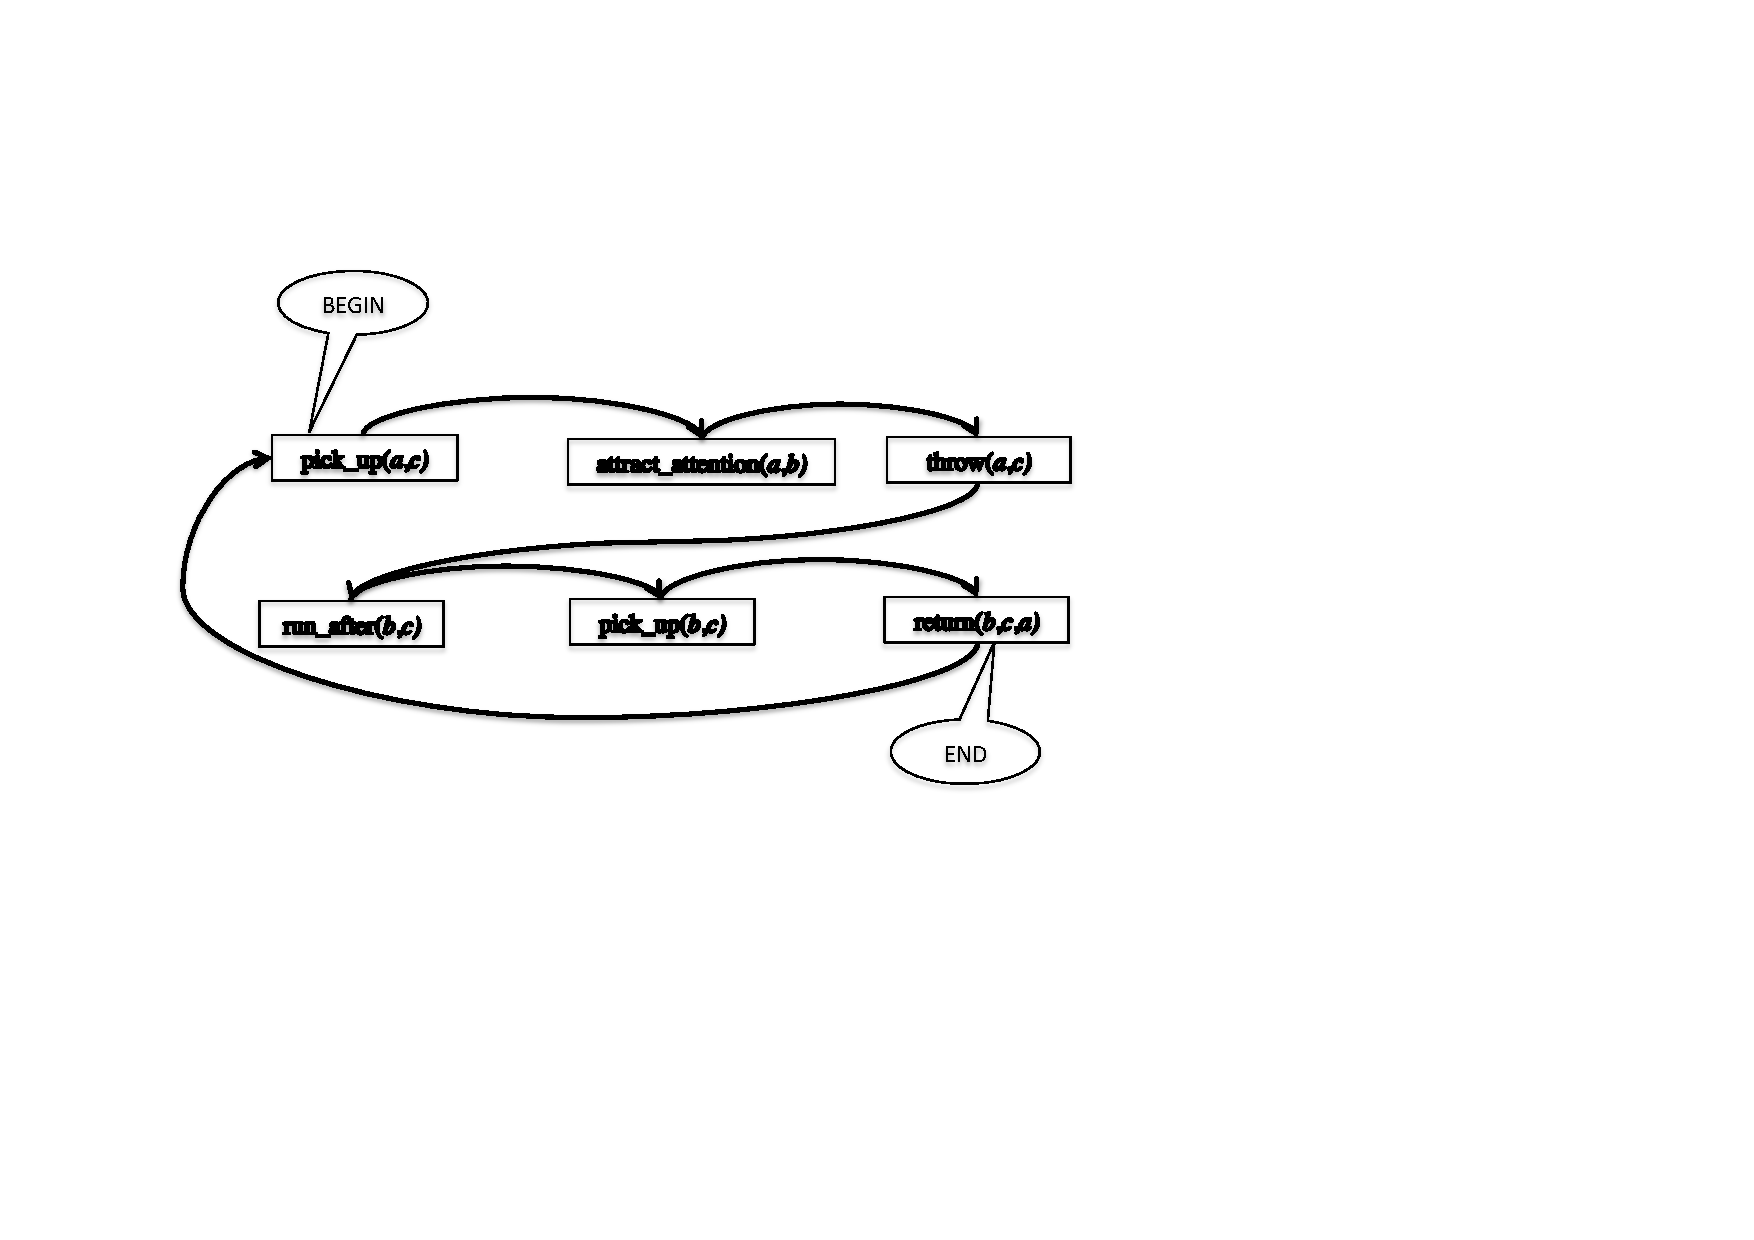
\includegraphics[width=6in]{fetch}

\hspace*{-4em}\begin{tikzpicture}[
  play/.style={rectangle, fill=Lamentation5, draw=Lamentation1, text=white, text depth=0.25ex, text height=1.5ex}
  ]

\node [play, pin=above:\textbf{Begin}] (p1) {pick\_up($a,c$)};
\node [play, right=of p1] (p2) {attract\_attention($a,b$)};
\node [play, right=of p2] (p3) {throw($a,c$)};
\node [play, below=1.5 of p1] (p4) {run\_after($b,c$)};
\node [play, right=of p4] (p5) {pick\_up($b,c$)};
\node [play, right=of p5, pin=below:\textbf{End}] (p6) {return($b,c,a$)};

\path [-{Stealth[]}, thick] 
(p1) edge [bend left] (p2)
(p2) edge [bend left] (p3)
(p3) edge [out=240, in=60] (p4)
(p4) edge [bend left] (p5)
(p5) edge [bend left] (p6)
(p6) edge [out=210, in=190, looseness=1.7] (p1);  
\end{tikzpicture}


\caption{play\_fetch($a$,$b$,$c$)}
\label{fig:fetch}
\end{figure}




   

In an important series of papers including
\cite{Fernando2004,Fernando2006,Fernando2008,Fernando2009,Fernando2011}, Fernando introduces a finite state
approach to event analysis where events are analyzed in terms of
finite state automata something like what we have represented in
Figure~\ref{fig:fetch-fs}.
\begin{figure} 

%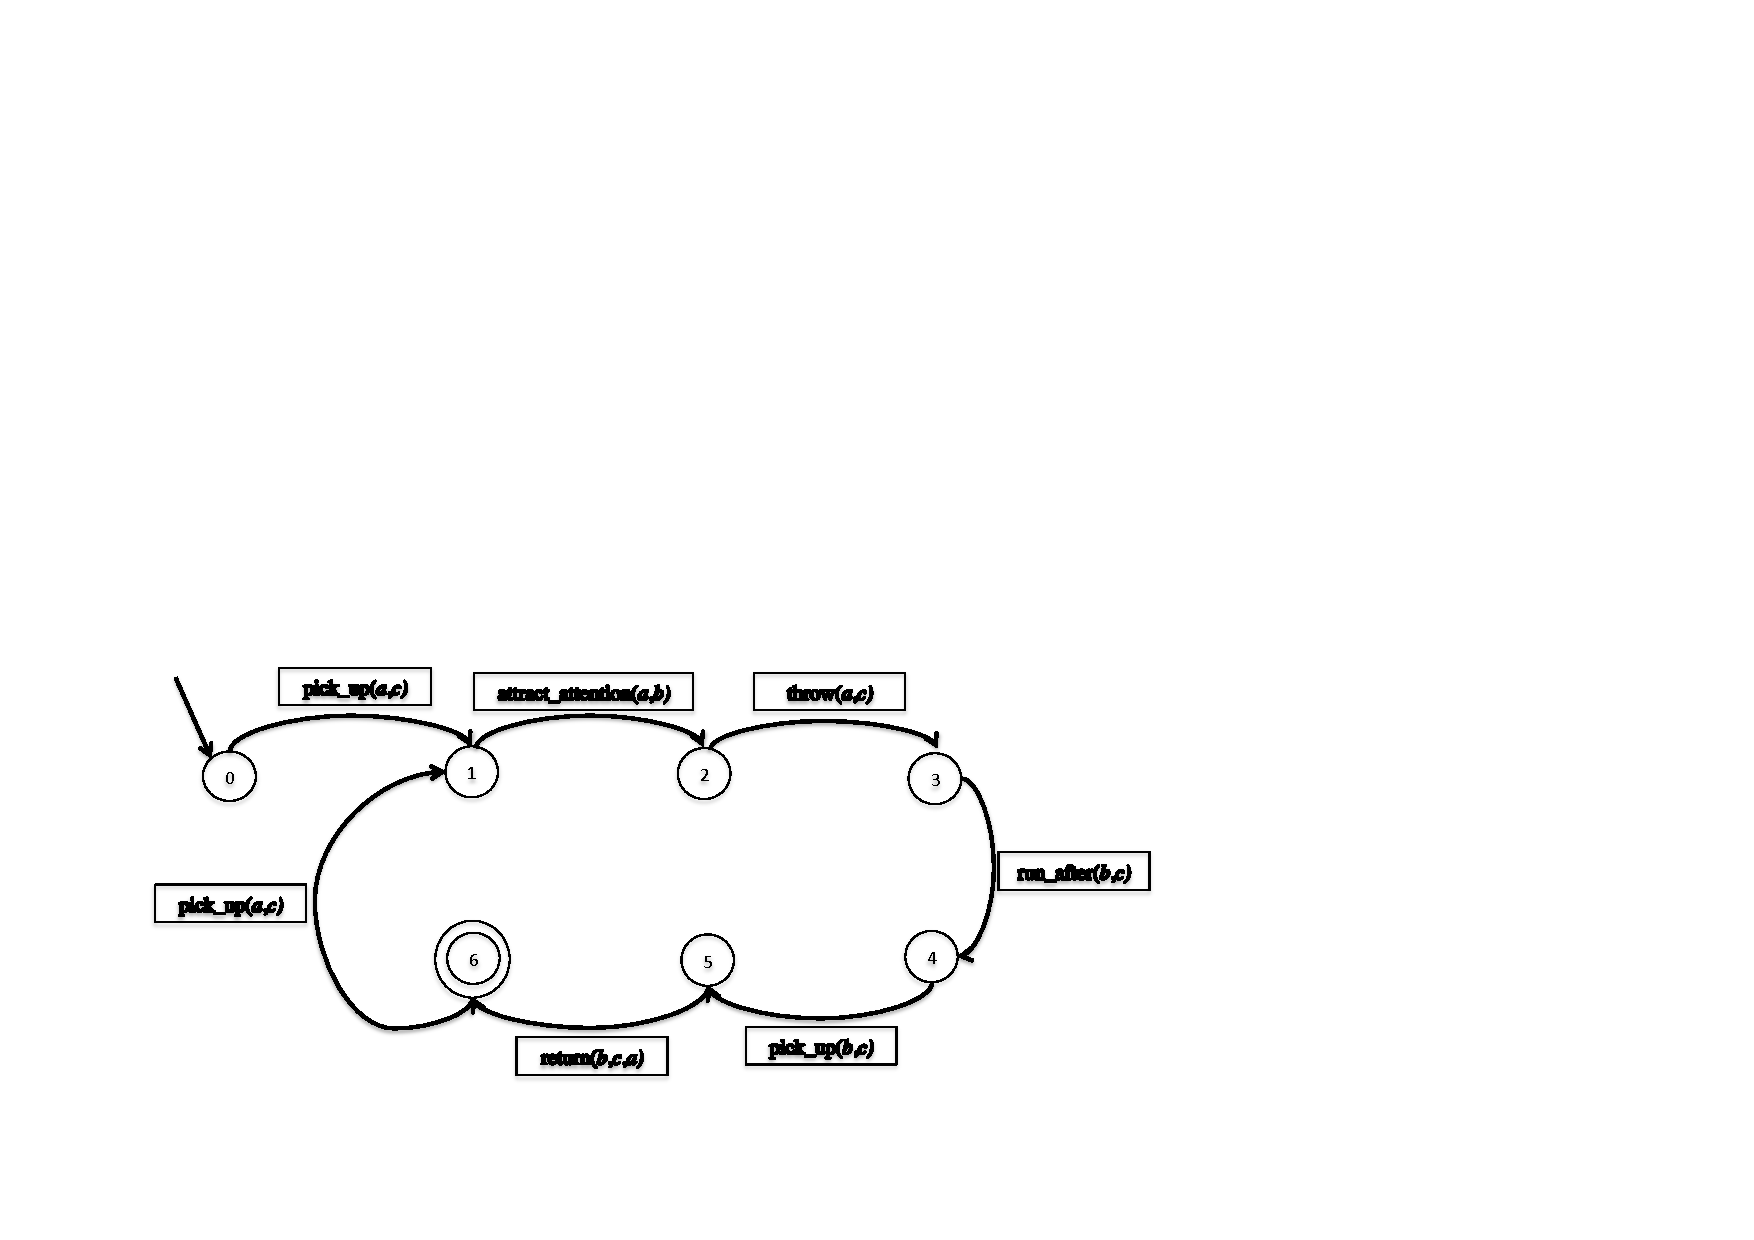
\includegraphics[width=6in]{fetch-fs}

\begin{tikzpicture}[
  node distance=3cm, 
  on grid,
  every state/.style={fill=Lamentation2},
  ]

\node [state, initial] (n0) {0};
\node [state] (n1) [right=of n0] {1};
\node [state] (n2) [right=of n1] {2};
\node [state] (n3) [right=of n2] {3};
\node [state] (n4) [below=of n3] {4};
\node [state] (n5) [left=of n4] {5};
\node [state, accepting] (n6) [left=of n5] {6};

\path [-{Stealth[]}, thick] 
(n0) edge [bend left] node [above] {pick\_up($a,c$)} (n1)
(n1) edge [bend left] node [above] {attract\_attention($a,b$)} (n2)
(n2) edge [bend left] node [above] {throw($a,c$)} (n3)
(n3) edge [bend left] node [right] {run\_after($b,c$)} (n4)
(n4) edge [bend left] node [below] {pick\_up($b,c$)} (n5)
(n5) edge [bend left] node [below] {return($b,c,a$)} (n6)
(n6) edge [bend left] node [left] {pick\_up($a,c$)} (n1);
\end{tikzpicture}


\caption{play\_fetch($a$,$b$,$c$) as a finite state machine}
\label{fig:fetch-fs}
\end{figure}  
Such an automaton will recognize a string of
sub-events.  The idea is that our perception of complex events can be seen as strings of
punctual observations similar to the kind of sampling we are
familiar with from audio technology and digitization processing in
speech recognition.  Thus events can be analyzed as strings of smaller
events.  What we mean by a string is made precise in
Appendix~\ref{sec:regular}. Any object of any type can be part of a
string.  Any two objects (including strings themselves), $s_1$ and $s_2$, can be
\textit{concatenated} to form a string ${s_1}^{\frown}s_2$.  An
important property of concatenation is \textit{associativity}, that is
if we concatenate $s_1$ with $s_2$ and then concatenate the result
with $s_3$ we get the same string that we would obtain by
concatenating $s_2$ with $s_3$ and then concatenating $s_1$ with the
result.  In symbols: $({s_1}^{\frown}s_2)^{\frown}s_3 =
{s_1}^{\frown}({s_2}^{\frown}s_3)$.  For this reason we normally write
${s_1}^{\frown}{s_2}^{\frown}s_3$ (without the parentheses) or simply
$s_1s_2s_3$ if it is clear from the context that we mean this to be
string concatenation.  Following Fernando we will use these strings to
give us our notion of temporal order. 

Although we will present strings in this way, we will model them as
records \label{pg:stringsasrecords} with distinguished labels related to the natural numbers, 
t$_0$, t$_1$, \ldots (`t' for ``time'').  The field labelled t$_n$
will correspond to the $n$th place in the string.  Thus a string of
objects $a_1a_2a_3$
will be the record in \nexteg{}.
\begin{ex} 
\record{\field{t$_0$}{$a_1$} \\
        \field{t$_1$}{$a_2$} \\
        \field{t$_2$}{$a_3$}} 
\end{ex} 
The concatenation of \preveg{} with the string $a_4$, that is, \nexteg{a}, will
be \nexteg{b}.
\begin{ex} 
\begin{subex} 
 
\item \record{\field{t$_0$}{$a_4$}} 
 
\item  \record{\field{t$_0$}{$a_1$} \\
        \field{t$_1$}{$a_2$} \\
        \field{t$_2$}{$a_3$} \\
        \field{t$_3$}{$a_4$}}
 
\end{subex} 
   
\end{ex} 
We will continue to
represent strings for convenience in the traditional way but modelling
strings as records will become important when following paths in
records down to elements in strings.  We will use $s[n]$ to represent
the $n$th element in a string $s$ (where the first element in the
string is $s[0]$).  But in terms of the record notation
this is just a convenient abbreviation for $s$.t$_n$.    

Now let us build further on the
types that we have introduced so far to include string types. For any
two types, $T_1$ and $T_2$, we can form the type ${T_1}^{\frown}T_2$.
This is the type of strings $a^{\frown}b$ where $a:T_1$ and $b:T_2$.
The concatenation operation on types (just like that on objects) is
associative so we do not use parentheses when more than one type is
involved, e.g. ${T_1}^{\frown}{T_2}^{\frown}T_3$.

Let us return to Kim watching the boy, $a$, playing fetch with the
dog, $b$, using the stick, $c$. % over a time interval $t$
She
perceives the event as being of type play\_fetch($a$,$b$,$c$).
But what does it mean to be an event of this type?  Given our
concatenation types we can build a type which corresponds to most of
what we have sketched in Figure~\ref{fig:fetch}, namely \nexteg{}.
% (again ignoring time for the sake of simplification).
\begin{ex} 
pick\_up($a$,$c$)$^{\frown}$attract\_attention($a$,$b$)$^{\frown}$throw($a$,$c$)$^{\frown}$run\_after($b$,$c$)$^{\frown}$pick\_up($b$,$c$)$^{\frown}$return($b$,$c$,$a$) 
\end{ex} 
\preveg{} is a type corresponding to everything we have represented in
Figure~\ref{fig:fetch} except for the arrow which loops back from the
end state to the start state.    In order to get the loop into the event
type we will use a kind of type which introduces a Kleene-+.  In
standard notations for strings $s^+$ stands for a string consisting of
one or more occurrences of $s$.\footnote{This notation was introduced
  by the mathematician Stephen Kleene.}  We will adopt this into types
by saying that for any type $T$ there is also a type $T^+$ which is
the type of strings of objects of type $T$ containing one or more
members.  (See Appendix~\ref{sec:regular} for a more precise
definition.)  The type \nexteg{} will, then,
give us a type corresponding to the complete Figure~\ref{fig:fetch}
since it will be the type consisting of strings of one or more events
of the type \preveg{}.
\begin{ex} 
(pick\_up($a$,$c$)$^{\frown}$attract\_attention($a$,$b$)$^{\frown}$throw($a$,$c$)$^{\frown}$run\_after($b$,$c$)$^{\frown}$pick\_up($b$,$c$)$^{\frown}$
\\ return($b$,$c$,$a$))$^+$ 
\end{ex}


% In \preveg{} we simplified the string type by excluding time.  Now we
% will consider what is needed to put time back in.  Each of the
% subevents represented there is associated with a time interval, a
% different time interval for each subevent.  The type for time
% intervals, which we will abbreviate as \textit{TimeInt} is \nexteg{}\label{pg:TimeInt}.
% \begin{ex} 
% \record{\tfield{start}{\textit{Time}} \\
%         \tfield{end}{\textit{Time}} \\
%         \tfield{c$_<$}{start$<$end}}
% \end{ex} 
% where \textit{Time} is the type of time points and $<$ is the relation
% ``earlier than'' defined on the witnesses of this type.\footnote{We
%   use the infix notation $t_1<t_2$ rather than the official notation
%   $<(t_1,t_2)$.}  In order to get time intervals associated with each
% subevent we will treat the subevent types as record types rather than
% ptypes.  Thus as a first step towards characterizing the right type we
% have \nexteg{}.
% \begin{ex} 
% \smallrecord{\smalltfield{e-time}{\textit{TimeInt}} \\
%              \smalltfield{c$_{\mathrm{pick\_up}}$}{pick\_up($a$,$c$,e-time)}}$^{\frown}$\smallrecord{\smalltfield{e-time}{\textit{TimeInt}}
%              \\
%                   \smalltfield{c$_{\mathrm{attract\_attention}}$}{attract\_attention($a$,$b$,e-time)}}$^{\frown}$

% \medskip
% \smallrecord{\smalltfield{e-time}{\textit{TimeInt}} \\
%              \smalltfield{c$_{\mathrm{throw}}$}{throw($a$,$c$,e-time)}}$^{\frown}$\smallrecord{\smalltfield{e-time}{\textit{TimeInt}} \\
%              \smalltfield{c$_{\mathrm{run\_after}}$}{run\_after($b$,$c$,e-time)}}$^{\frown}$

% \medskip
% \smallrecord{\smalltfield{e-time}{\textit{TimeInt}} \\
%              \smalltfield{c$_{\mathrm{pick\_up}}$}{pick\_up($b$,$c$,e-time)}}$^{\frown}$\smallrecord{\smalltfield{e-time}{\textit{TimeInt}} \\
%              \smalltfield{c$_{\mathrm{return}}$}{return($b$,$c$,$a$,e-time) }}
% \end{ex}

% This will get us a time interval for each subevent but it does not
% require any relationship between the time intervals of the different
% subevents whereas, of course, each subevent should occur at a later
% time than the previous one.  In order to achieve this we will
% introduce a more restricted notion of type concatenation especially
% for record types which have a field
% \smallrecord{\smalltfield{e-time}{\textit{TimeInt}}} as in \nexteg{}.
% \begin{ex}
% \begin{enumerate} 
% \item If $T_1$ and $T_2$ are subtypes of
% \smallrecord{\smalltfield{e-time}{\textit{TimeInt}}}$^+$ then
% $T_1^{\frown_<}T_2$ is a type. 

% \item $a:T_1^{\frown_<}T_2$ iff $a=a_1^{\frown}a_2$, $a_1:T_1$, $a_2:T_2$ and
%   last($a_1$).e-time.end$<$first($a_2$).e-time.start
% \end{enumerate}
% \end{ex} 
% Here first($s$) and last($s$) pick out the first and last elements
% respectively of the string $s$.  We need to make a similar adjustment
% to the Kleene-+ type constructor.
% \begin{ex} 
% \begin{enumerate} 
 
% \item If $T$ is a subtype of
%   \smallrecord{\smalltfield{e-time}{\textit{TimeInt}}} then $T^{+_<}$
%   is a type
 
% \item $a:T^{+_<}$ iff $a=x_1^\frown\!\ldots^\frown\!x_n$, $n>0$ and
%   for $i$, $j$, $1\leq
% i<j\leq n$, $x_i:T$, $x_j:T$ and $x_i^{\frown}x_j:T^{\frown_<}T$ 
 
% \end{enumerate} 
   
% \end{ex} 

% [The details of temporal concatenation above should be included in the
% appendix.]

We will complicate \preveg{} slightly by substituting record types for
the ptypes as in \nexteg{}.  We do this because we
will want to allow for things happening simultaneously and record
types will give us a straightforward way of allowing this.
\begin{ex} 
(\smallrecord{\smalltfield{e}{pick\_up($a$,$c$)}}$^{\frown}$\smallrecord{\smalltfield{e}{attract\_attention($a$,$b$)}}$^{\frown}$\smallrecord{\smalltfield{e}{throw($a$,$c$)}}$^{\frown}$\smallrecord{\smalltfield{e}{run\_after($b$,$c$)}}$^{\frown}$\\
\smallrecord{\smalltfield{e}{pick\_up($b$,$c$)}}$^{\frown}$\smallrecord{\smalltfield{e}{return($b$,$c$,$a$)}})$^+$ 
\label{eg:fetch-type}
\end{ex}
The label `e' (``event'') occurs in each of the elements of the string
type.  In this case we will say that `e' labels a \textit{dimension}
of events of this type.  The `e'-dimension can be thought of as the
dimension which characterizes what is happening at each stage of the
event.  If you want to think geometrically, you can think of the
event-string as being located in a space of event types (that is, the ptypes).

% So now we can represent the event type for playing fetch as \nexteg{}.
% \begin{ex} 
% (\smallrecord{\smalltfield{e-time}{\textit{TimeInt}} \\
%              \smalltfield{c$_{\mathrm{pick\_up}}$}{pick\_up($a$,$c$,e-time)}}$^{\frown_<}$\smallrecord{\smalltfield{e-time}{\textit{TimeInt}}
%              \\
%                   \smalltfield{c$_{\mathrm{attract\_attention}}$}{attract\_attention($a$,$b$,e-time)}}$^{\frown_<}$

% \medskip
% \smallrecord{\smalltfield{e-time}{\textit{TimeInt}} \\
%              \smalltfield{c$_{\mathrm{throw}}$}{throw($a$,$c$,e-time)}}$^{\frown_<}$\smallrecord{\smalltfield{e-time}{\textit{TimeInt}} \\
%              \smalltfield{c$_{\mathrm{run\_after}}$}{run\_after($b$,$c$,e-time)}}$^{\frown_<}$

% \medskip
% \smallrecord{\smalltfield{e-time}{\textit{TimeInt}} \\
%              \smalltfield{c$_{\mathrm{pick\_up}}$}{pick\_up($b$,$c$,e-time)}}$^{\frown_<}$\smallrecord{\smalltfield{e-time}{\textit{TimeInt}} \\
%              \smalltfield{c$_{\mathrm{return}}$}{return($b$,$c$,$a$,e-time) }})$^{+_<}$
% \end{ex}

What happens when Kim perceives an event as being of this type?  She
makes a series of observations of events, assigning them to types in
the string type.  Note that the ptypes in each of the types can be
further broken down in a similar way.  This gives us a whole hierarchy
of perceived events which at some point have to bottom out in basic
perceptions which are not further analyzed.  In order to recognize an
event as being of this type Kim does not need to perceive a string of
events corresponding to each of the types in the string types.  She
may, for example, observe the boy waving the stick to attract the
dog's attention, get distracted by a bird flying overhead for a while,
and then return to the fetch event at the point where the dog is
running back to the boy with the stick.  This still enables her to
perceive the event as an event of fetch playing because she has seen
such events before and learned that such events are of the string type in \preveg{}.  It suffices for her to observe enough of the elements in
the string to distinguish the event from other event types she may
have available in her knowledge resources.  Suppose, for example, that
she has just two event string types available that begin with the picking
up of a stick by a human in the company of a dog.  One is \preveg{}.
The other is one that leads to the human beating the dog with the
stick.  If she only observes the picking up of the stick she cannot be
sure whether what she is observing is a game of fetch or a beating.
However, as soon as she observes something in the event string which
belongs only to the fetch type of string she can reasonably conclude
that she is observing an event of the fetch type.  She may, of course,
be wrong.  She may be observing an event of a type which she does not
yet have available in her resource of event types, in which case she
will need to learn about the new event type and add it to her
resources.  However, given the resources at her disposal she can make
a prediction about the nature of the rest of the event.  One could
model her prediction making ability in terms of a function which maps
a situation (modelled as a record) to a type of predicted situation,
for example \nexteg{}.
\begin{ex} 
$\lambda r$:\smallrecord{\smalltfield{x}{\textit{Ind}} \\
                         \smalltfield{c$_{\mathrm{human}}$}{human(x)}
                         \\
                         \smalltfield{y}{\textit{Ind}} \\
                         \smalltfield{c$_{\mathrm{dog}}$}{dog(y)} \\
                         \smalltfield{z}{\textit{Ind}} \\
                         \smalltfield{c$_{\mathrm{stick}}$}{stick(z)}
                         \\
                         \smalltfield{e}{\smallrecord{
             \smalltfield{e}{pick\_up(x,z)}}$^{\frown}$\smallrecord{
                  \smalltfield{e}{attract\_attention(x,y)}}}} .
            \\*[.75\baselineskip]
\hspace*{4em}\smallrecord{\smalltfield{e}{play\_fetch($r$.x,$r$.y,$r$.z)}
\\
\smalltfield{c$_{\mathrm{init}}$}{init($r$.e,e)}}
\label{ex:ev-predict-fun}
\end{ex} 
% \begin{ex} 
% $\lambda r$:\smallrecord{\smalltfield{x}{\textit{Ind}} \\
%                          \smalltfield{c$_{\mathrm{human}}$}{human(x)}
%                          \\
%                          \smalltfield{y}{\textit{Ind}} \\
%                          \smalltfield{c$_{\mathrm{dog}}$}{dog(y)} \\
%                          \smalltfield{z}{\textit{Ind}} \\
%                          \smalltfield{c$_{\mathrm{stick}}$}{stick(z)}
%                          \\
%                          \smalltfield{e-time}{\textit{TimeInt}} \\
%                          \smalltfield{e}{\smallrecord{\smalltfield{e-time}{\textit{TimeInt}}
%                              \\
% \smalltfield{c$_{\leq}$}{$\Uparrow$e-time.start$\leq$e-time.start} \\
%              \smalltfield{c$_{\mathrm{pick\_up}}$}{pick\_up($\Uparrow$x,$\Uparrow$z,e-time)}}$^{\frown_<}$\smallrecord{\smalltfield{e-time}{\textit{TimeInt}}
%              \\
% \smalltfield{c$_{\leq}$}{e-time.start$\leq\Uparrow$e-time.start} \\
%                   \smalltfield{c$_{\mathrm{attract\_attention}}$}{attract\_attention($\Uparrow$x,$\Uparrow$y,e-time)}}}}
%             \\*[.75\baselineskip]
% \hspace*{4em}(\smallrecord{\smalltfield{e-time}{\textit{TimeInt}} \\
%                            \smalltfield{c$_{\leq}$}{$r$.e-time.start$\leq$e-time.start} \\
%                            \smalltfield{e}{play\_fetch($r$.x,$r$.y,$r$.z,e-time)}})
% \label{ex:ev-predict-fun}
% \end{ex}

Here the predicate `init' has arity
$\langle$\textit{String}, \textit{String}$\rangle$.  The type init($s_1$,$s_2$) is
non-empty just in case $s_1$ is an initial substring of $s_2$.  We
achieve this by defining
\begin{quote}
If $s_1$ is a string of length $n$ and $s_2$ is a string of any
length, then $s$ : init($s_1$,$s_2$) iff the length of $s_2$ is
greater than or equal to $n$ and for each $i$, $0\leq i<n$,
$s_1[i]=s_2[i]$ and $s=s_2$.
\end{quote}
That is, if the initial substring condition holds then the second
argument to the predicate (and nothing else) is of the ptype.

% Here a `$\Uparrow$' prefixed to a path-name consisting of labels such
% as `e-time.start' or `x' means that the path-name is to start in the
% next higher record type in which the current record type is embedded.
% This notation is an abbreviation for something much less readable (but
% more precise) which is given in Appendix~\ref{app:rectypes}. [????
% This notation needs to be added to the appendix.]

The kind of function of which \preveg{} is an instance is a function
of the general form \nexteg{}.
\begin{ex} 
$\lambda a\!:\!T_1\ .\ T_2(a)$
\label{ex:deptypefun} 
\end{ex} 
where we use the notation $T_2(a)$ to represent the fact that $T_2$
depends on $a$. The nature of this dependence in
(\ref{ex:ev-predict-fun}) is seen in the occurrences of $r$ in the body
of the function, for example, `play\_fetch($r$.x,$r$.y,$r$.z)'.
Such a function maps an object of some type (represented by $T_1$) to
a type (represented by $T_2(a)$).  The type that results from an
application of this function will depend on what object it is applied
to -- that is, we have the possibility of obtaining different types
from different objects. In type theory such a function is often called
a \textit{dependent type}.  These functions will play an important
role in much of what is to come later in this book.  They will show up
many times in what appear at first blush to be totally unrelated
phenomena.  We want to suggest, however, that all of the phenomena we
will describe using such functions have their origin in our basic
cognitive ability to make predictions on the basis of partial
observation of objects and events.

What happens when Kim does not observe enough of the event to be able
to predict with any certainty that the complete event will be a game
of fetch?  One theory would be that she can only make categorical
judgements, and that she has to wait until she has seen enough so that
there is only one type that matches in the collection of situation
types in her resources.  Another theory would be
one where she predicts a disjunction of the available matching types when there is
more than one that matches.  One might refine this theory so that she
can choose one of the available types but assign it a probability
based on the number of matching types.  If $n$ is the number of
matching types the probability of any one of them might be
$\frac{1}{n}$.  This assumes that each of the types is equally likely
to be realized.  It would be natural to assume, however, that the
probability which Kim assigns to any one of the matching types would
be dependent on her previous experience.  Suppose, for example, that
she has seen 100 events of a boy picking up a stick in the company of
a dog, 99 of those events led to a game of fetch and only one led to
the boy beating the dog.  One might then assume that when she now sees
the boy pick up the stick she would assign a 99\% probability to the
type of fetch events and only 1\% probability to the boy beating the
dog.  That is, the probability she assigns to an event of a boy
picking up a stick leading to a game of fetch is the result of
dividing the number of instances of a game of fetch she has already
observed by the sum of the number of instances she has observed of any types whose
initial segment involves the picking up of a stick.  In more general
terms we can compute the probability which an agent $A$ assigns on the
basis of a string, $\omega$, of previous observations to a
predicted type $T_{\mathit{pr}}$ given an observed type $T_{\mathit{obs}}$, $P_{A,\omega}(T_{\mathit{pr}}\mid T_{\mathit{obs}})$, in the case where
$T_{\mathit{pr}}$ is a member of the set of alternatives which can be
predicted from $T_{\mathit{obs}}$ according to $A$'s resources based on $\omega$,
$\mathrm{alt}_{A,\omega}(T_{\mathit{obs}})$, by the following formula:
\[P_{A,\omega}(T_{\mathit{pr}}\mid T_{\mathit{obs}}) =
\frac{\mid\{T_{\mathit{pr}}\}^{A,\omega}\mid}{\sum\limits_{T_{\mathit{alt}}\in\mathrm{alt}_{A,\omega}(T_{\mathit{obs}})}\mid\{T_{\mathit{alt}}\}^{A,\omega}\mid}\]
where $\{T\}^{A,\omega}$ is the set of objects of type $T$ observed by $A$
in $\omega$.  If $T_{\mathit{pr}}$ is not a member of
$\mathrm{alt}_{A,\omega}(T_{\mathit{obs}})$, that is not one of the
alternatives, we say that $P_{A,\omega}(T_{\mathit{pr}}\mid
T_{\mathit{obs}}) = 0$.

While this is still a rather naive and simple view of how
probabilities might be assigned it is not without interest, as shown
by the following points:  
\paragraph{Probability distributions} It will always provide a probability distribution over sets
of alternatives, that is,
\[\sum\limits_{T_{\mathit{pr}}\in\mathrm{alt}_{A,\omega}(T_{\mathit{obs}})}P_{A,\omega}(T_{\mathit{pr}}\mid
T_{\mathit{obs}}) = 1\]
\paragraph{Alternatives} We have assumed a notion of alternatives based on types of completed
events for which the observed event is an initial segment but other
notions of alternativeness could be considered and perhaps even
combined.  
\paragraph{Relativity of probability assignments} The notion of
probability is both agent and resource relative.  It represents the
probability which an agent will assign to a type when observing a
given situation after a previous string of observations.  Two agents may assign different
probabilities depending on the resources they have available.
\paragraph{Learning} Relevant observations will update the probability
distributions an agent will assign to a given set of alternatives
since the probability is computed on the basis of previous
observations of the alternative types.

Kim is not alone in being able to draw conclusions based on partial
observations of an event.  The dog can do it too.  As soon as the boy
has raised the stick and attracted the dog's attention the dog is
excitedly snapping at the stick and starting to run in the direction
in which the boy seems to be about to throw.  The dog also seems to be
attuned to string types of events just as Kim is and also able to make
predictions on the basis of partial observations.  The types to which
a dog is attuned will not be the same as those to which humans can be
attuned and this can certainly lead to miscommunication between humans
and dogs.  For example, there may be many reasons why I would go to
the place where outdoor clothes are hanging and where the dog's lead
is kept.  Many times it will be because I am planning to take the dog
out for a walk, but not as often as the dog appears to think, judging
from the excitement he shows any time I go near the lead.  It is
difficult to explain to the dog that I am just looking for a receipt
that I think I might have left in my coat pocket.  But the basic
mechanism of being able to assemble types of events
into string types of more complex events and make predictions on the
basis of these types seems to be common to both humans and dogs and a
good number of other animals too.  Perhaps simple organisms do not
have this ability and can only react to events that have already
happened, but not to predicted outcomes.

This basic inferential ability is thus not parasitic on the ability to
communicate using a human language.  It is, however, an ability which
appears to be exploited to a great extent in our use of language as we
will see in later chapters.  In the remaining sections of this chapter
we will look at some aspects of the type theory which seem more likely
to
correspond to cognitive abilities which only humans have.


% When talking about the intuition behind this
% analysis Fernando sometimes refers to strings of frames in a movie
% (e.g. in \cite{Fernando2008}).  But in many cases what he is calling
% a movie frame 
% can also be seen as a frame in something like the sense of frame semantics as well.

\section{Doing things with types}
\label{sec:typeacts}

The boy and the dog have to coordinate and interact in order to create an
event of the game of fetch.  This involves doing more with types than
just making judgements.  For example, when the dog observes the
situation in which the boy raises the stick, it may not be clear
to the dog whether this is part of a fetch-game situation or a
stick-beating situation.  The dog may be in a situation of
entertaining these two types as possibilities prior to making the
judgement that the situation is of the fetch type.  We will call this
act a query as opposed to a judgement.  Once the dog has made the
judgement that what it has observed so far is an initial segment of a
fetch type situation it has to make its own contribution in order to
realize the fetch type, that is, it has to run after the stick and
bring it back.  This involves the creation of a situation of a certain
type.  Thus creation acts are another kind of act related to types.
Creating objects of a given type often has a \textit{de se}
\citep[see, for example,][]{Perry1979,Lewis1979a,Ninan2010,Schlenker2011} aspect.  The dog
has to know that it itself must run after the stick in order to make
this a situation in which it and the boy are playing fetch.  There is
something akin to what Perry calls an essential indexical here,
though, of course, the dog does not have indexical linguistic
expressions. It is nevertheless part of the basic competence that an
agent needs in order to be able to coordinate its action with the rest
of the world that it has a primitive sense of self which is distinct
from being able to identify an object which has the same properties as
itself.  We will follow Lewis in modelling \textit{de se} in terms of
functional abstraction over the ``self''.  In our terms this will mean
that \textit{de se} type acts involve dependent types.

In standard type theory we have judgements such as $o:T$ ``$o$ is of type $T$'' 
and 
$T$ \textit{true} ``there is something of type $T$''.    We want to
enhance this notion of judgement by including a reference to the agent
$A$ which makes the judgement, giving judgements such as
$o:_AT$ ``agent $A$ judges that $o$ is of type $T$''
and 
$:_AT$ ``agent $A$ judges that there is some object of type $T$''. We will call
the first of these a \textit{specific} judgement and the second a
\textit{non-specific} judgement.  Such
judgements are one of the three kinds of acts represented in \nexteg{}
that we want to include
in our type act theory.
\begin{ex} 
\textit{Type Acts}
\begin{description}
\item[judgements] \mbox{}

\begin{description}
\item[\textit{specific}] $o:_A T$ ``agent $A$ judges object $o$ to be of type
  $T$''

\item[\textit{non-specific}] $:_A T$ ``agent $A$ judges that there is some
  object of type $T$''
\end{description}

\item[queries] \mbox{}
\begin{description}
\item[\textit{specific}] $o:_A T?$ ``agent $A$ wonders whether object $o$ is of type
  $T$''

\item[\textit{non-specific}] $:_A T?$ ``agent $A$ wonders whether there is some object of type
$T$''
\end{description}
\item[creations] \mbox{}
\begin{description}
\item[\textit{non-specific}] $:_A T!$ ``agent $A$ creates something of type
  $T$''
\end{description}
\end{description}

\end{ex} 
Note that creations only come in the non-specific variant.  You cannot
create an object which already exists.  

Creations are also limited in
that there are certain types which a given agent is not able to
realize as the main actor.  Consider for example the event type involved in the fetch
game of the dog running after the stick.  The human cannot be the main
creator of such
an event since it is the dog who is the actor.  The most the human can
do is wait until the dog has carried out the action
and we will count this as a creation type act.  This will become
important when we discuss coordination in the fetch-game below.  It is
actually important that the human makes this passive contribution to
the creation of the event of the dog running after the stick and does
not, for example, get the game confused by immediately throwing
another stick before the dog has had a chance to retrieve the first
stick.  There are other cases of event types which require a less
passive contribution from an agent other than the main actor.
Consider the type of event where the dog returns the stick to the
human.  The dog is clearly the main actor here but the human has also
a role to play in making the event realized.  For example, if the
human turns her back on the dog and ignores what is happening or runs
away the event type will not be realized despite the dog's best
efforts.  Other event types, such as lifting a piano, involve more
equal collaboration between two or more agents, where it is not
intuitively clear that any one of the agents is the main actor.  So
when we say ``agent $A$ creates something of type $T$'' perhaps it
would be more accurate to phrase this as ``agent $A$ contributes to
the creation of something of type $T$'' where $A$'s contribution might
be as little as  not realizing any of the other types involved in the game until
$T$ has been realized.   
   
\textit{De se} type acts involve functions which have the agent in its
domain and return a type, that is, they are dependent types which,
given the agent, will yield a type.  We will say that agents are of
type \textit{Ind} and that the relevant dependent types, 
$\mathcal{T}$, are functions of type
  (\textit{Ind}$\rightarrow$\textit{Type}).  
We characterize \textit{de se} type acts in a way parallel to
\preveg{}, as given in \nexteg{}.
\begin{ex}
\textit{De Se Type Acts} 
\begin{description}
\item[\textit{judgements}] \mbox{}
\begin{description}
\item[\textit{specific}]  $o:_A \mathcal{T}(A)$ ``agent $A$ judges object $o$ to be of type
  $\mathcal{T}(A)$''
\item[\textit{non-specific}] $:_A \mathcal{T}(A)$ ``agent $A$ judges
  that there is some object of type $\mathcal{T}(A)$''
\end{description}

\item[\textit{queries}] \mbox{}
\begin{description}
\item[\textit{specific}] $o:_A \mathcal{T}(A)?$ ``agent $A$ wonders whether object $o$ is of type
  $\mathcal{T}(A)$''
\item[\textit{non-specific}] $:_A \mathcal{T}(A)?$ ``agent $A$ wonders whether there is some object of type
$\mathcal{T}(A)$''
\end{description}

\item[\textit{creations}] \mbox{}
\begin{description}
\item[\textit{non-specific}] $:_A \mathcal{T}(A)!$ ``agent $A$ creates
  something of type $\mathcal{T}(A)$''
\end{description}
\end{description} 
\end{ex} 

From the point of view of the type theory \textit{de se} type acts
seem more complex than non-\textit{de se} type acts since they involve
a dependent rather than a non-dependent type and a functional
application of that dependent type to the agent.  However, from a
cognitive perspective one might expect \textit{de se} type acts to be
more basic.  Agents which perform type acts using types directly
related to themselves are behaving egocentrically and one could regard
it as a more advanced level of abstraction to consider types which are
independent of the agent.  This seems a puzzling way in which our
notions of type seem in conflict with out intuitions about cognition.   

While these type acts are prelinguistic (we need them to account for
the dog's behaviour in the game of fetch) we will try to argue later
that they are the basis on which the notion of speech act
\citep{Austin1962,Searle1969} is built.  Our notion of using types in
query acts seems intuitively related to work on inquisitive semantics
\citep{GroenendijkRoelofsen2012} where some propositions (in
particular disjunctions) are regarded as inquisitive.  However, this
will still allow us to make a distinction between questions and
assertions in natural language as argued for by \cite{Ginzburg2012}.

Let us now apply these notions to the kind of interaction that has to
take place between the human and the dog in a game of fetch.  First
consider in more detail what is actually involved in playing a game of
fetch, that is creating an event of type (\ref{eg:fetch-type}).  Each
agent has to keep track in some way of where they are in the game and
in particular what needs to happen next.  We analyze this by saying
that each agent has an information state which we will model as a
record.  We need to keep track of the progression of types of
information state for an agent during the course of the game.  We will
refer to the types of information states as gameboards.\footnote{Our
  notions of \textit{information state} and \textit{gameboard} are
  taken from \cite{Larsson2002} and \cite{Ginzburg2012} respectively
  as well as a great deal of related literature on the gameboard or
  information state approach to dialogue analysis originating from
  \cite{Ginzburg1994}.  We have adapted the notions somewhat to our own
  purposes and will take this up in more detail in
  Chapter~\ref{ch:infex}.}  The idea is that as part of the event
occurs then the agent's gameboard is updated so that an event of the
next type in the string is expected.  For now, we will consider
gameboards which only place one requirement on information states,
namely that there is an agenda which indicates the type of the next
move in the game.  Thus if the agent is playing fetch and observes an
event of the type where the human throws the stick, then, according to
(\ref{eg:fetch-type}), the next move in the game will be an event of
the type where the dog runs after the stick.  If the actor in the next
move is the agent herself then the agent will need to create an event
of the type of the next move if the game is to progress.  If the actor in the next move is the
other player in the game, then the agent will need to observe an event
and judge it to be of the appropriate type in order for the game to
progress.  The type of information states, \textit{InfoState}, will be
\nexteg{a}.  (In Chapter~\ref{ch:infex}, when we apply these ideas to dialogue, we
will see more complex information states.)  The type of the initial
information state, \textit{InitInfoState}, will be one where the agenda is required to be the
empty list.
\begin{ex}
\begin{subex} 
\item \record{\tfield{agenda}{[\textit{RecType}]}}
\item \record{\mfield{agenda}{[]}{[\textit{RecType}]}} 
\end{subex}
\end{ex} 
We can now see the rules of the game corresponding to the type
(\ref{eg:fetch-type}) as a set of update functions which indicate for
an information state of a given type what type the next information
state may belong to if an event of a certain type occurs.  These
update functions correspond to the transitions in a finite state
machine.  This is
given in \nexteg{}.
\begin{ex} 
\{ \begin{tabular}[t]{l}
$\lambda
  r$:\smallrecord{\smallmfield{agenda}{[]}{[\textit{RecType}]}} . \\
\hspace*{1em}\smallrecord{\smallmfield{agenda}{[\smallrecord{\smalltfield{e}{pick\_up($a$,$c$)}}]}{[\textit{RecType}]}},
\\ 
$\lambda
r$:\smallrecord{\smallmfield{agenda}{[\smallrecord{\smalltfield{e}{pick\_up($a$,$c$)}}]}{[\textit{RecType}]}}
\\
\hspace*{1em}$\lambda
e$:\smallrecord{\smalltfield{e}{pick\_up($a$,$c$)}} . \\
\hspace*{2em}\smallrecord{\smallmfield{agenda}{[\smallrecord{\smalltfield{e}{attract\_attention($a$,$b$)}}]}{[\textit{RecType}]}},
\\
$\lambda
r$:\smallrecord{\smallmfield{agenda}{[\smallrecord{\smalltfield{e}{attract\_attention($a$,$b$)}}]}{[\textit{RecType}]}}
\\
\hspace*{1em}$\lambda
e$:\smallrecord{\smalltfield{e}{attract\_attention($a$,$b$)}} . \\
\hspace*{2em}\smallrecord{\smallmfield{agenda}{[\smallrecord{\smalltfield{e}{throw($a$,$c$)}}]}{[\textit{RecType}]}},
\\
$\lambda
r$:\smallrecord{\smallmfield{agenda}{[\smallrecord{\smalltfield{e}{throw($a$,$c$)}}]}{[\textit{RecType}]}}
\\
\hspace*{1em}$\lambda
e$:\smallrecord{\smalltfield{e}{throw($a$,$c$)}} . \\
\hspace*{2em}\smallrecord{\smallmfield{agenda}{[\smallrecord{\smalltfield{e}{run\_after($b$,$c$)}}]}{[\textit{RecType}]}},
\\
$\lambda
r$:\smallrecord{\smallmfield{agenda}{[\smallrecord{\smalltfield{e}{run\_after($b$,$c$)}}]}{[\textit{RecType}]}}
\\
\hspace*{1em}$\lambda
e$:\smallrecord{\smalltfield{e}{run\_after($b$,$c$)}} . \\
\hspace*{2em}\smallrecord{\smallmfield{agenda}{[\smallrecord{\smalltfield{e}{pick\_up($b$,$c$)}}]}{[\textit{RecType}]}},
\\
$\lambda
r$:\smallrecord{\smallmfield{agenda}{[\smallrecord{\smalltfield{e}{pick\_up($b$,$c$)}}]}{[\textit{RecType}]}}
\\
\hspace*{1em}$\lambda
e$:\smallrecord{\smalltfield{e}{pick\_up($b$,$c$)}} . \\
\hspace*{2em}\smallrecord{\smallmfield{agenda}{[\smallrecord{\smalltfield{e}{return($b$,$c$,$a$)}}]}{[\textit{RecType}]}},
\\
$\lambda
r$:\smallrecord{\smallmfield{agenda}{[\smallrecord{\smalltfield{e}{return($b$,$c$,$a$)}}]}{[\textit{RecType}]}}
\\
\hspace*{1em}$\lambda
e$:\smallrecord{\smalltfield{e}{return($b$,$c$,$a$)}} . \\
\hspace*{2em}\smallrecord{\smallmfield{agenda}{[]}{[\textit{RecType}]}}
\\
% $\lambda
% r$:\smallrecord{\smallmfield{agenda}{[\smallrecord{\smalltfield{e}{return($b$,$c$,$a$)}}]}{[\textit{RecType}]}}
% \\
% \hspace*{1em}$\lambda
% e$:\smallrecord{\smalltfield{e}{return($b$,$c$,$a$)}} . \\
% \hspace*{2em}\smallrecord{\smallmfield{agenda}{[\smallrecord{\smalltfield{e}{[pick\_up($a$,$c$)]}}]}{[\textit{RecType}]}}
 \end{tabular} \\
\hspace*{\textwidth} \} 
\label{eg:fetch-update-funs} 
 
   
\end{ex} 

Since we are treating an empty agenda as the condition for the input
to the initial state in the corresponding automaton and also the
output of the final state we automatically get the loop effect from
the final state to the initial state.  In order to prevent the loop we
would have to distinguish the type corresponding to the initial and
final states. Note that the functions in \preveg{} are of the
type \nexteg{}.
\begin{ex}
(\smallrecord{\smalltfield{agenda}{[\textit{RecType}]}}$\rightarrow$(\textit{Rec}$\rightarrow$\textit{RecType}))
\end{ex}
That is, they map an information state containing an agenda (modelled
as a record containing an agenda field) and an
event (modelled as a record) to a record type.   This is true of all
except for the function corresponding to the initial state which is of
type \nexteg{}.
\begin{ex}
(\smallrecord{\smalltfield{agenda}{[\textit{RecType}]}}$\rightarrow$\textit{RecType})
\end{ex}
That is, it maps an information state directly to a record type and does not
require an event.  We can think of this set as the set of rules which
define the game.  It is of the type \nexteg{}.
\begin{ex}
\{((\smallrecord{\smalltfield{agenda}{[\textit{RecType}]}}$\rightarrow$(\textit{Rec}$\rightarrow$\textit{RecType}))$\vee$(\smallrecord{\smalltfield{agenda}{[\textit{RecType}]}}$\rightarrow$\textit{RecType}))\}
\end{ex}
Let us call the type in \preveg{} \textit{GameRules}.  Sets of game
rules of this type define the rules for specific participants as in
(\ref{eg:fetch-update-funs}).  In order to characterize the game in
general we need to abstract out the roles of the individual
participants in the game.  This we will do by defining a function from
a record containing individuals appropriate to play the roles in the
game thus revising (\ref{eg:fetch-update-funs}) to \nexteg{}.

\begin{ex}
$\lambda r^*$:\record{\tfield{h}{\textit{Ind}} \\
                          \tfield{c$_{\mathrm{human}}$}{human(h)} \\
                          \tfield{d}{\textit{Ind}} \\
                          \tfield{c$_{\mathrm{dog}}$}{dog(d)} \\
                          \tfield{s}{\textit{Ind}} \\
                          \tfield{c$_{\mathrm{stick}}$}{stick(s)}}
                        . \\ 
\hspace*{1em}\{ \begin{tabular}[t]{l}
$\lambda
  r$:\smallrecord{\smallmfield{agenda}{[]}{[\textit{RecType}]}} . \\
\hspace*{1em}\smallrecord{\smallmfield{agenda}{[\smallrecord{\smalltfield{e}{pick\_up($r^*$.h,$r^*$.s)}}]}{[\textit{RecType}]}},
\\ 
$\lambda
r$:\smallrecord{\smallmfield{agenda}{[\smallrecord{\smalltfield{e}{pick\_up($r^*$.h,$r^*$.s)}}]}{[\textit{RecType}]}}
\\
\hspace*{1em}$\lambda
e$:\smallrecord{\smalltfield{e}{pick\_up($r^*$.h,$r^*$.s)}} . \\
\hspace*{2em}\smallrecord{\smallmfield{agenda}{[\smallrecord{\smalltfield{e}{attract\_attention($r^*$.h,$r^*$.d)}}]}{[\textit{RecType}]}},
\\
$\lambda
r$:\smallrecord{\smallmfield{agenda}{[\smallrecord{\smalltfield{e}{attract\_attention($r^*$.h,$r^*$.d)}}]}{[\textit{RecType}]}}
\\
\hspace*{1em}$\lambda
e$:\smallrecord{\smalltfield{e}{attract\_attention($r^*$.h,$r^*$.d)}} . \\
\hspace*{2em}\smallrecord{\smallmfield{agenda}{[\smallrecord{\smalltfield{e}{throw($r^*$.h,$r^*$.s)}}]}{[\textit{RecType}]}},
\\
$\lambda
r$:\smallrecord{\smallmfield{agenda}{[\smallrecord{\smalltfield{e}{throw($r^*$.h,$r^*$.s)}}]}{[\textit{RecType}]}}
\\
\hspace*{1em}$\lambda
e$:\smallrecord{\smalltfield{e}{throw($r^*$.h,$r^*$.s)}} . \\
\hspace*{2em}\smallrecord{\smallmfield{agenda}{[\smallrecord{\smalltfield{e}{run\_after($r^*$.d,$r^*$.s)}}]}{[\textit{RecType}]}},
\\
$\lambda
r$:\smallrecord{\smallmfield{agenda}{[\smallrecord{\smalltfield{e}{run\_after($r^*$.d,$r^*$.s)}}]}{[\textit{RecType}]}}
\\
\hspace*{1em}$\lambda
e$:\smallrecord{\smalltfield{e}{run\_after($r^*$.d,$r^*$.s)}} . \\
\hspace*{2em}\smallrecord{\smallmfield{agenda}{[\smallrecord{\smalltfield{e}{pick\_up($r^*$.d,$r^*$.s)}}]}{[\textit{RecType}]}},
\\
$\lambda
r$:\smallrecord{\smallmfield{agenda}{[\smallrecord{\smalltfield{e}{pick\_up($r^*$.d,$r^*$.s)}}]}{[\textit{RecType}]}}
\\
\hspace*{1em}$\lambda
e$:\smallrecord{\smalltfield{e}{pick\_up($r^*$.d,$r^*$.s)}} . \\
\hspace*{2em}\smallrecord{\smallmfield{agenda}{[\smallrecord{\smalltfield{e}{return($r^*$.d,$r^*$.s,$r^*$.h)}}]}{[\textit{RecType}]}},
\\
$\lambda
r$:\smallrecord{\smallmfield{agenda}{[\smallrecord{\smalltfield{e}{return($r^*$.d,$r^*$.s,$r^*$.h)}}]}{[\textit{RecType}]}}
\\
\hspace*{1em}$\lambda
e$:\smallrecord{\smalltfield{e}{return($r^*$.d,$r^*$.s,$r^*$.h)}} . \\
\hspace*{2em}\smallrecord{\smallmfield{agenda}{[]}{[\textit{RecType}]}}
\\
% $\lambda
% r$:\smallrecord{\smallmfield{agenda}{[\smallrecord{\smalltfield{e}{return($b$,$c$,$a$)}}]}{[\textit{RecType}]}}
% \\
% \hspace*{1em}$\lambda
% e$:\smallrecord{\smalltfield{e}{return($b$,$c$,$a$)}} . \\
% \hspace*{2em}\smallrecord{\smallmfield{agenda}{[\smallrecord{\smalltfield{e}{[pick\_up($a$,$c$)]}}]}{[\textit{RecType}]}}
 \end{tabular} \\
\hspace*{\textwidth} \} 
\end{ex}
\preveg{} is of type (\textit{Rec}$\rightarrow$\textit{GameRules})
which we will call \textit{Game}. 
  
Specifying the rules of the game in terms of update functions in this way will not actually getting
anything to happen, though.  For that we need type acts of the kind we
discussed. We link the update functions to type acts by means of
\textit{licensing conditions on type acts}.  A basic licensing
condition is that an agent can create (or contribute to the creation
of) a witness for the first type that occurs on the agenda in its
information state.  Such a licensing condition is expressed in
\nexteg{}.
\begin{ex} 
If $A$ is an agent, $s_i$ is $A$'s current information state, \\ $s_i
:_A$ \record{\mfield{agenda}{$T\!\mid\!
    R\ $}{[\textit{RecType}]}}, then $:_A T!$ is licensed. 
\end{ex}
(Here we use the notation $T\!\mid\!R$ to represent a list whose first
member is $T$ and whose rest is $R$.  For example, if the list is
$[T_1,T_2,T_3]$ then $T$ would correspond to $T_1$ and $R$ would
correspond to $[T_2,T_3]$. See Appendix~\ref{app:listtypes}.) 

Update functions of the kind we have discussed are handled by the
licensing conditions in \nexteg{}.
\begin{ex} 
\begin{subex} 
 
\item If $f:(T_1\rightarrow(T_2\rightarrow\textit{Type}))$ is an update
function, $A$ is an agent, $s_i$ is $A$'s current information state,
$s_i:_A T_i$, $T_i\sqsubseteq T_1$ (and $s_i:T_1$), then an event $e:_A
T_2$ (and $e:T_2$) licenses $s_{i+1}:_A f(s_i)(e)$. 
 
\item If $f:(T_1\rightarrow(T_2\rightarrow\textit{Type}))$ is an update
function, $A$ is an agent, $s_i$ is $A$'s current information state,
$s_i:_A T_i$, $T_i\sqsubseteq T_1$ (and $s_i:T_1$), $s_{i+1}:_A
f(s_i)$ is licensed. 
 
\end{subex} 
   
\end{ex} 
\preveg{a} is for the case where the update function requires an event in
order to be triggered and \preveg{b} is for the case where no event is
required. There are two variants of licensing conditions which can be
considered.  One variant is where the licensing conditions rely only
on the agent's judgement of information states and events occurring.
The other variant is where in addition we require that the information
states and events actually are of the types which the agent judges
them to be of.  (These conditions are represented in parentheses in
\preveg{}.)  In practical terms an agent has to rely on its own
judgement, of course, and there is one sense in which any resulting
action is licensed even if the agent's judgement was mistaken.  There
is another stricter sense of license which requires the agent's
judgement to be correct.  In the real world, though, the only way we
have of judging a judgement to be correct is to look at judgements by
other agents.

Licensing conditions will regulate the coordination of
successfully realized games like fetch.  They enable the agents to
coordinate their activity when they both have access to the same
objects of type \textit{Game} and are both willing to play.  The use
of the word ``license'' is important, however.  The agents have free
will and may choose not to do what is licensed and also may perform
acts that are not licensed.  We cannot build a theory that will
predict exactly what will happen but we can have a theory which tells
us what kinds of actions belong to a game.  It is up to the agents to
decide whether they will play the game or not.  At the same time,
however, we might regard whatever is licensed at a given point in the
game as an obligation.  That is, if there is a general obligation to
continue a game once you have embarked on it, then whatever type is
placed on an agent's agenda as the result of a previous event in the
game can be seen as an obligation on the agent to play its part in the
creation of an event of that type.



 

\section{Modal type systems}
\label{sec:percint-modal}

Kim continues her walk still thinking about the boy and the dog.  She
thinks,  ``Was
the boy standing too close to the pond?  Suppose he had fallen in.  If
he had been my son, I wouldn't have let him play just there.'' An
important aspect of human cognition is that we are not only able to
observe things as they are but also to conceive of alternatives which
go beyond the completion of observed events in the way discussed in
Section~\ref{sec:ev-strings}. We can not only observe objects and
perceive them to be of certain types we can also consider
possibilities in which they belong to different types and perhaps do
not belong to the type we have observed.  We have managed to unhook
type judgements from direct perception.  While the seeds of this
ability can be seen in the kind of event perception and prediction
discussed above in that it gives us a way to consider types which have
not yet been realized, it is at least one step further in cognitive
evolution to be able to consider alternative type assignments which do
not correspond to completions of events already perceived.

% While perception and typing are at the core of cognitive processing an
% important feature of cognitive systems is the ability to consider
% alternative typings which have not be observed. 

% While we perceive $a$ to
% be of type $T_1$ it is perhaps nevertheless conceivable that $a$ could
% have been of type $T_2$.

This leads us to construct \textit{modal type
systems} with alternative assignments of objects to
types.\footnote{The term \textit{modal} is taken from modal logic. See
  \cite{HughesCresswel1968} for a classic introduction. A modern
  introduction is to be found in \cite{BlackburnRijkeVenema2001}.}
Figure~\ref{fig:modal} provides an example of a modal system of basic
types with two
possibilities, one where the extensions of types $T_1$ and $T_2$
overlap and another possibility where they do not.  

\begin{figure}[h]
%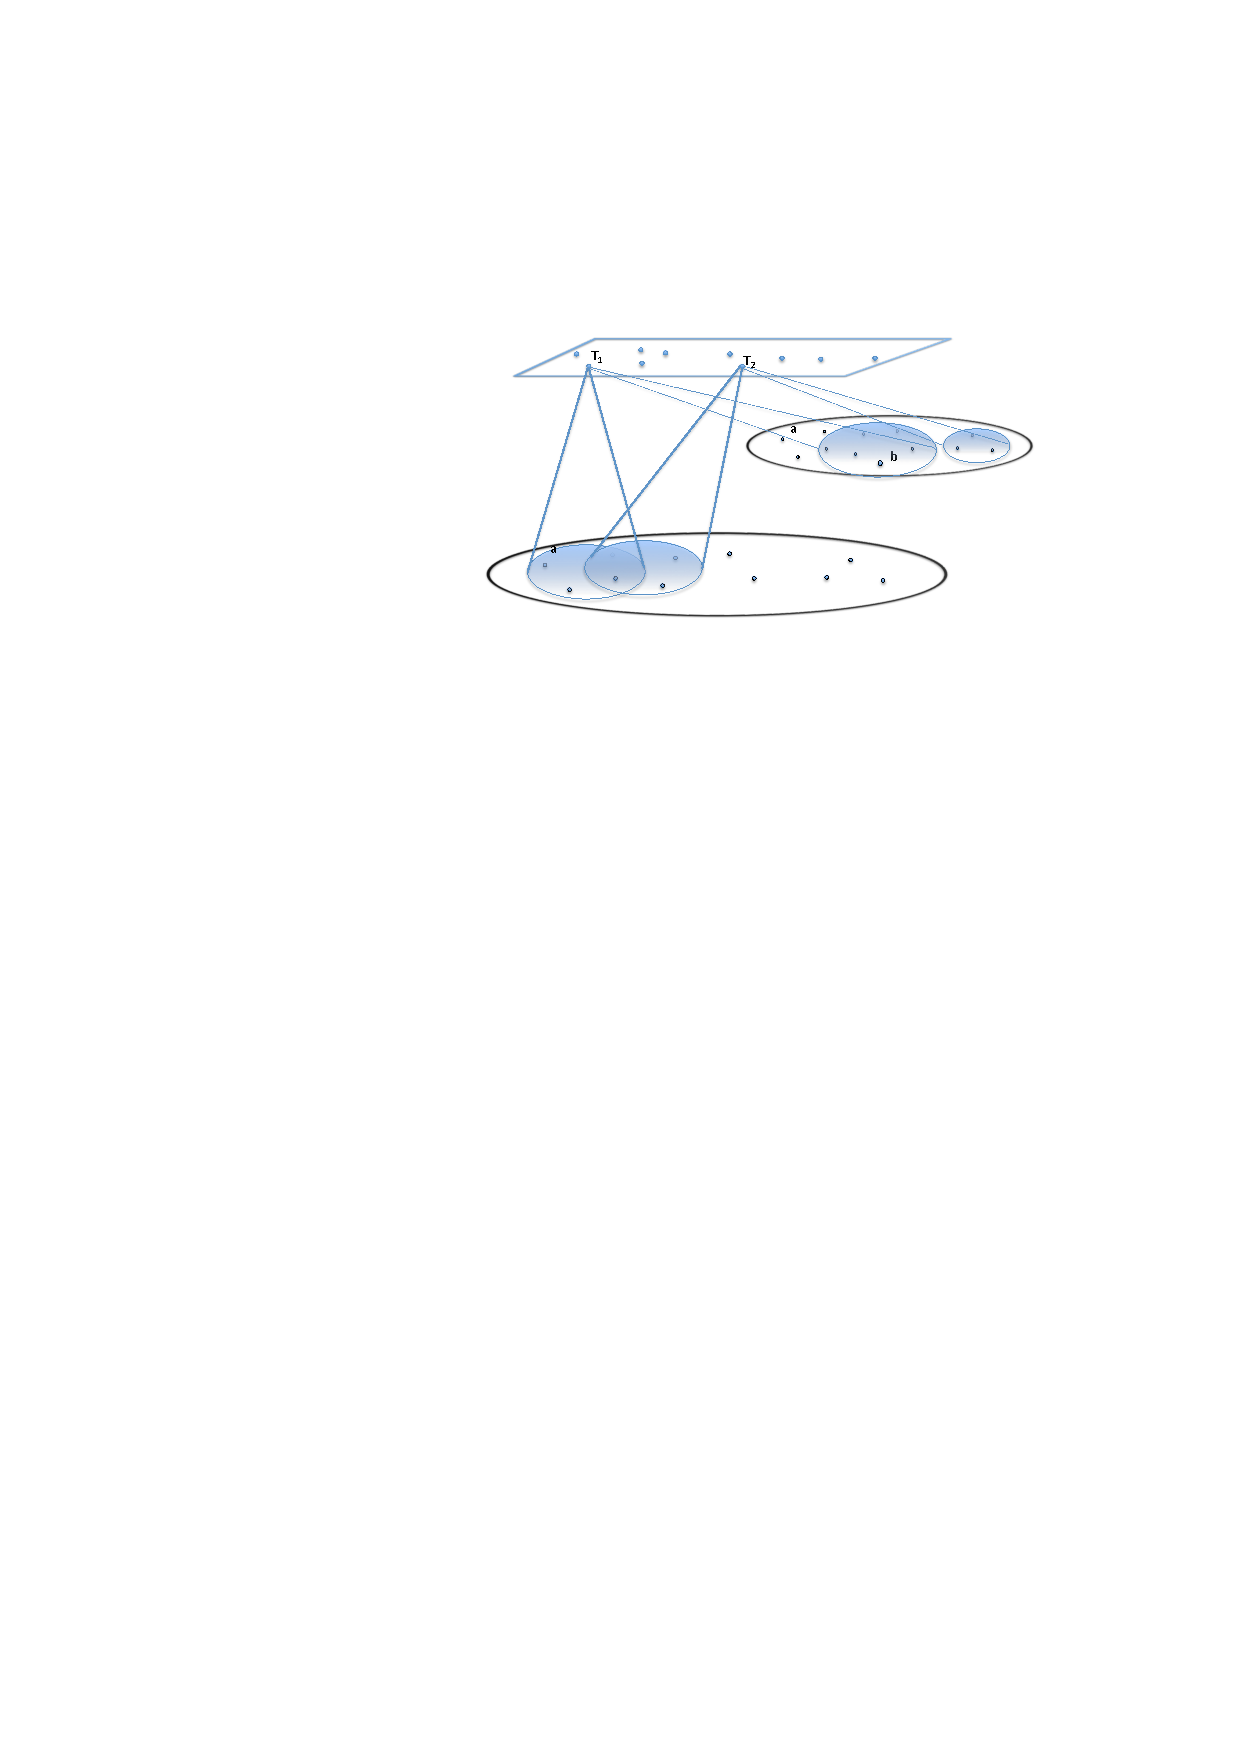
\includegraphics[width=\textwidth]{modal}
\begin{adjustbox}{max width=\textwidth}
\begin{tikzpicture}[
  type/.style={circle, inner sep=0pt, minimum size=6pt, ball color=BTypeCol},
  firsttype/.style={circle, inner sep=0pt, minimum size=6pt, ball color=FirstTypeCol},
  secondtype/.style={circle, inner sep=0pt, minimum size=6pt, ball color=SecondTypeCol},
  objects/.style={circle, inner sep=0pt, minimum size=6pt, ball color=ObjectCol},
  modalobjects/.style={circle, inner sep=0pt, minimum size=6pt, ball color=ModalCol}
  ]

  % basic types:
  \begin{scope}[
    % every node/.append style={yslant=0,xslant=1.75},
    yslant=0,xslant=1.75
    ]
    \filldraw [fill=BTypeCol, draw=BorderCol, thick, fill opacity=0.5] (0,0) rectangle (8,2);

    \foreach \x/\y in {0.5/1.3, 1.4/1.6, 1.8/1.3, 1.9/0.5, 3.3/1.8, 2.6/1.5, 4.4/0.9, 4.7/1, 5.5/0.3, 5.6/1.1, 5.5/1.7, 6.4/1.2, 6.7/1.6} {
      \node [type] at (\x,\y) {};
    }

    \node [coordinate] (btypeleft) at (0,1) {};
    \node [coordinate] (btyperight) at (8,1) {};

    \node [type, label=above:$T_1$] (t1) at (1.3,0.6) {};
    \node [type, label=above:$T_2$] (t2) at (4.5,0.5) {};
  \end{scope}    


  % objects:
  \begin{scope}[
    % every node/.append style={yslant=0,xslant=1.75},
    %yslant=0,xslant=1.75,
    yshift=-100
    ]
    \filldraw [fill=ObjectCol, opacity=0.4, draw=BorderCol, ultra thick] (5,0) ellipse (6 and 1);

    \foreach \a/\b in {5.5/0.7, 6.4/0.2, 6.7/0.6, 7/0, 7.5/0.35, 8/-0.3, 8.1/0.2, 8.7/0, 9/0.2, 10/0.1} {
      \node [objects] at (\a,\b) {};
    }
    % for T1 from BType:
    \node [modalobjects, label=above:$a$] (o1) at (0.3,-0.1) {}; 
    \node [objects] (o2) at (1,0.35) {}; 
    \node [objects] (o3) at (1.6,-0.2) {};
    \node [ellipse, fit=(o1) (o2) (o3), yscale=0.7, draw=BTypeCol, thick, fill=BTypeCol, fill opacity=0.3] (fitA) {};
    \draw [BTypeCol, thick] (t1) -- (fitA.east);
    \draw [BTypeCol, thick] (t1) -- (fitA.west);

    % for T2 from BType:
    \node [objects] (o4) at (2.6,-0.5) {};
    \node [objects] (o5) at (3.1,-0.5) {};
    \node [objects] (o6) at (3.3,-0.1) {};
    \node [ellipse, fit=(o3) (o4) (o5) (o6), yscale=0.7, draw=BTypeCol, thick, fill=BTypeCol, fill opacity=0.2] (fitB) {};
    \draw [BTypeCol, thick] (t2) -- (fitB.east);
    \draw [BTypeCol, thick] (t2) -- (fitB.west);

    % % for T2 from Type1:
     \node [objects] (o7) at (4,0.4) {};
     \node [objects] (o8) at (4.4,0) {}; 
     \node [objects] (o9) at (4.7,0.1) {};
    % \node [ellipse, fit=(o3) (o4) (o5) (o6) (o7) (o8) (o9), yscale=0.6, xscale=0.9, draw=FirstTypeCol, thick, fill=FirstTypeCol, fill opacity=0.2] (fitC) {};

    % % for T2 from Type2:
     \node [objects] (o10) at (5.5,-0.3) {};
     \node [objects] (o11) at (5.6,-0.1) {};
    % \node [ellipse, fit=(o3) (o4) (o5) (o6) (o7) (o8) (o9) (o10) (o11), yscale=0.7, xscale=0.8, draw=SecondTypeCol, thick, fill=SecondTypeCol, fill opacity=0.2] (fitD) {};
  \end{scope}


  % modal types:
  \begin{scope}[
    % every node/.append style={yslant=0,xslant=1.75},
    %yslant=0,xslant=1.75,
    yshift=-35, 
    xshift=220
    ]
    \filldraw [fill=ObjectCol, opacity=0.4, draw=BorderCol, ultra thick] (3.5,0) ellipse (4 and 0.75);

    \foreach \a/\b in {0.3/-0.1, 1.5/-0.3, 3.9/0.2, 7/0} {
      \node [objects] at (\a,\b) {};
    }
    \node [modalobjects, label=above:$a$] at (0.7,0) {};
    \node [objects] (i1) at (5.7,-0.2) {};
    \node [objects] (i2) at (6.1,0.3) {};
    \node [objects] (i3) at (5,0) {};
    \node [ellipse, fit=(i1) (i2) (i3), yscale=0.7, draw=BTypeCol,
    thick, fill=BTypeCol, fill opacity=0.2] (fitAA) {};
    \draw [BTypeCol, thick] (t2) -- (fitAA.north);
    \draw [BTypeCol, thick] (t2) -- (fitAA.south west);

    \node [objects] (i4) at (1.6,0.1) {};
    \node [objects] (i5) at (2,0.2) {};
    \node [modalobjects, label=above:$b$] (i6) at (2.5,-0.3) {};
    \node [objects] (i7) at (2.7,0.35) {};
    \node [ellipse, fit=(i4) (i5) (i6) (i7), yscale=0.7, xscale=1.1,
    draw=BTypeCol, thick, fill=BTypeCol, fill opacity=0.2] (fitBB) {};
    \draw [BTypeCol, thick] (t1) -- (fitBB.north);
    \draw [BTypeCol, thick] (t1) -- (fitBB.south west);
  \end{scope}


  % % Type1:
  % \begin{scope}[
  %   % every node/.append style={yslant=0,xslant=1.75},
  %   yslant=0,xslant=1.75,
  %   xshift=-100,
  %   yshift=80
  %   ]
  %   \filldraw [fill=FirstTypeCol, draw=BorderCol, thick, fill opacity=0.3] (0,0) rectangle (8,2);
  %   \node [coordinate] (firsttypeleft) at (0,1) {};
  %   \node [coordinate] (firsttyperight) at (8,1) {};

  %   \foreach \x/\y in {0.45/1.4, 1.4/1.6, 1.9/0.5, 3.3/1.8, 2.6/1.5, 4.7/1, 5.5/0.3, 5.6/1.1,  6.7/1.6} {
  %     \node [firsttype] at (\x,\y) {};
  %   }

  %   \node [firsttype, label=above:$T_1$] (ft1) at (1.8,1.1) {};
  %   \node [firsttype, label=above:$T_2$] (ft2) at (5.8,0.7) {};
  %   \node [firsttype, label=above:$T_3$] (ft3) at (6.4,1.2) {};
  %   \node [firsttype, label=above:{\textbf{Type$^1$}}] (ft) at (4,0.4) {};

  %   \draw [FirstTypeCol, thick] (ft) -- (btypeleft);
  %   \draw [FirstTypeCol, thick] (ft) -- (btyperight);
    
  %   \draw [FirstTypeCol, thick] (ft2) -- (fitC.east);
  %   \draw [FirstTypeCol, thick] (ft2) -- (fitC.west);
  % \end{scope}    


  % % Type2:
  % \begin{scope}[
  %   % every node/.append style={yslant=0,xslant=1.75},
  %   yslant=0,xslant=1.75,
  %   xshift=-200,
  %   yshift=160
  %   ]
  %   \filldraw [fill=SecondTypeCol, draw=BorderCol, thick, fill opacity=0.1] (0,0) rectangle (8,2);
  %   \foreach \x/\y in {1.4/1.6, 1.9/0.5, 3.2/1.5, 4.7/1, 5.4/1.2, 5.8/0.3, 6/0.3,  6.2/1.6} {
  %     \node [secondtype] at (\x,\y) {};
  %   }

  %   \node [secondtype, label=above:$T_1$] (st1) at (1.2,1) {};
  %   \node [secondtype, label=above:$T_2$] (st2) at (4.8,0.7) {};
  %   \node [secondtype, label=above:$T_3$] (st3) at (2.6,1.3) {};
  %   \node [secondtype, label=above:{\textbf{Type$^2$}}] (st) at (3.4,0.5) {};

  %   \draw [SecondTypeCol, thick] (st) -- (firsttypeleft);
  %   \draw [SecondTypeCol, thick] (st) -- (firsttyperight);
    
  %   \draw [SecondTypeCol, thick] (st2) -- (fitD.east);
  %   \draw [SecondTypeCol, thick] (st2) -- (fitD.west);
  % \end{scope}    
\end{tikzpicture}
\end{adjustbox}

\caption{Modal system of basic types}
\label{fig:modal}
\end{figure}
The object $a$ is
of type $T_1$ in the first possibility but not in the second
possibility.  There is an object, $b$, of type $T_1$ in the second
possibility.  $b$ does not exist at all in the first possibility.
In the
figure we just show two possibilities but our general definition in Appendix~\ref{sec:basic}
allows for there to be any number of possibilities, including
infinitely many.

Given this apparatus we define four simple modal notions:
\begin{description}

\item[(necessary) equivalence] Two types are (necessarily) equivalent
  just in case the extension of one type is identical with that of
  the other type in all the possibilities.  While the different
  possibilities may provide different extensions for the types, it
  will always be the case that in any given possibility the two types
  will have the same extension.

\item[subtype] One type is a subtype of another just in case whatever
  possibility you look at it is always the case that the extension of
  the first type is a subset of the extension of the second.  We can
  also say that the first type ``entails'' the second, that is, any
  object which is of the first type will also be of the second type,
  no matter which possibility you are considering.

\item[necessity] The notion of necessity we characterize for a type
  could be glossed as ``necessarily realized'' or ``necessarily
  instantiated''.  A type will be necessary just in case there is
  something of the type in all the possibilities.

\item[possibility] This notion corresponds to ``possibly realized'' or
  ``possibly instantiated''.  A type will be possible just in case
  there is some possibility according to which it has a non-null
  extension.

\end{description}
These notions are made precise in Appendix~\ref{sec:basic}.  Note that
all of these notions are relativized to the modal system you are
considering and the possibilities it offers.  We may think of the
family of assignments $\mathcal{A}$ as providing a modal base
(cf. Kratzer) or alternatives (in the sense of ????).  For these kinds
of applications we may wish to consider very small families of
assignments corresponding to the knowledge we have.  Alternatively, we
may want to consider strong logical variants of these modal notions
where we consider all the logical possibilities, for example, all
possible assignments of extensions to types.

So far we have talked about modal systems of basic types.  Modal
systems of complex types, where we introduce ptypes, create a
minor complication.  What ptypes that are present in a system depends
on what objects there are of the types that are used in the arities of
the predicates.  Thus if we have some predicate $r$ with arity
$\langle\textit{Ind},\textit{Ind}\rangle$ and a possibility where the
set assigned to \textit{Ind} is $\{a,b\}$ then according to that
possibility the ptypes formed with $r$ will be $r(a,a)$, $r(a,b)$,
$r(b,a)$ and $r(b,b)$.  In a possibility where \textit{Ind} is
assigned a different set the set of available ptypes will be
different.  It is an important feature of type theories with types
constructed from predicates that the collection of such types depends
on what objects are available as arguments to the predicates.  This
makes type theory very different from a logical language such as
predicate calculus where the notion of well-formedness of syntactic
expressions containing predicates is defined independently of what is
provided by the model as denotations of arguments to the predicate.

This leads us (in Appendix~\ref{app:modal}) to define two variants of
each of our modal notions: \textit{restrictive} variants which are only defined
for types which exist in all possibilities and \textit{inclusive}
variants which require that the modal definition holds for all the
possibilities in which the types exist and disregards those in which
the types do not exist.  For example, a type is \textit{necessary}$_r$
(that is, ``restrictively necessary'') just in case the type is
available in all possibilities and has a non-empty set of witnesses in
all possibilities.  It is \textit{necessary}$_i$ (``inclusively
necessary'') just in case in all the possibilities in which the type
is provided it has a non-empty set of witnesses.  It is clear that if
a type is necessary$_r$ it will also be necessary$_i$ but there may be
types which are necessary$_i$ but not necessary$_r$ (if the type is
not provided in all possibilities).  A similar relationship between
the restrictive and inclusive notions holds for all the modal notions
we have discussed.

There may be significant classes of modal type systems in which the
types available in the different possibilities do not vary.  This
could be achieved by requiring that the types used in the arities of
predicates always have the same witnesses in all the possibilities.
This seems feasible if we restrict the types used in predicate arities
to basic ontological categories such as individual or time point.  It
seems reasonable to consider modal systems in which an individual in
one possibility will be an individual in any other possibility, for
example.  It seems reasonable to say that we wish to consider
possibilities where, for example, Kim is a man rather than a woman,
but not possibilities where Kim is a point in time rather than an
individual.  However, the notion ``basic ontological category'' is a
slippery one and we do not want to be forced to make commitments about that.

In the definition of a system of complex types in
section~\ref{app:comptypes}  we call the pair of an assignment to
basic types and assignment to ptypes, $\langle A,F\rangle$, a \textit{model} because of its
similarity to first order models.\footnote{For a more detailed
  discussion of the relationship between this and first order models
  as used in the interpretation of first order logic see
  \cite{Cooperforthcoming}.} The model provides an interface
between 
the type theoretical system and a domain external to the type theory.
The natural domain to relate to the type theory is that of individuals
and situations, that is the kind of things we can perceive or at least
consider as possibilities.  However, we may want to use models which
relate to our perceptual apparatus, as in \cite{Larsson2011}, rather
than directly to the world.  This can also be the key for relating the
type theory to a dynamically changing world where the models
representing our perceived possibilities are not fixed.  % We will
% return to this in Chapter~\ref{ch:coord}.



\section{Intensionality: propositions as types}

Kim continues to think about the boy and the dog as she walks along.
It was fun to see them playing together.  They seemed so happy.  The
boy obviously thought that the dog was a good playmate.  Kim is not
only able to perceive events as being of certain types.  She is able
to recall and reflect on these types.  She is able to form attitudes
towards these types: it was fun that the boy and the dog were playing but
a little worrying that they were so close to the pond.  This means
that the types themselves seem to be arguments to predicates like
`fun' and `worrying'.  This seems to be an important human ability --
not only to be able to take part in or observe an event and find it
fun or worrying but to be able to reflect independently of the actual
occurrence of the event that it or in general similar events are fun
or worrying.  This is a source of great richness in human cognition in
that it enables us to consider situation types independently of their
actual instantiation.\footnote{This richness also has its downside in
  that we often become so engaged in our internal cognitive abstraction
  that it can be difficult to be fully present and conscious of our
  direct perception of the world -- for example, worrying about what
  might happen in the future rather than enjoying the present.}  This
abstraction also enables us to consider what attitudes other
individuals might have.  For example, Kim believes that the boy
thought that the dog was a good playmate.  She is able to ascribe this
belief to the boy.  Furthermore, we are able to reflect on Kim's state
of mind where she has a belief concerning the type of situation where
the boy thinks that the dog was a good playmate.  And somebody else
could consider of us that we have a certain belief about Kim
concerning her belief about the boy's belief.  There
is in principle no limit to the depth of recursion concerning our
attitudes towards types.

We propose to capture this reflective nature of human cognition by
making the type theory technically \textit{reflective} in the sense
that we
allow types themselves to be objects which can belong to other types.
In classical model theoretic semantics we think of
\textit{believe} as corresponding to a relation between individuals
and propositions.  In our type theory, however, we are subscribing to
the ``propositions as types'' view which comes to us via
\cite{Martin-Loef1984} but has its origins in intuitionistic logic
[????].  Propositions are true or false.  Types of situations such as
hug($a$,$b$) correspond to propositions in the sense that if they are
non-empty then the proposition is true. If there is nothing of this
type then it is false.  The reasoning is thus that we do not need
propositions in our system as separate semantic objects if we already
have types.  We can use the types to play the role of propositions.
To believe a type is to believe it to be non-empty.  From the point of view
of a type theory for cognition in which we connect types to our basic
perceptual ability, this provides a welcome link between our perceptual
ability and our ability to entertain propositions (that is,  to
consider whether they are
true or false).

A predicate like `believe' which represents that an individual has an
attitude (of belief) to a certain type should thus have an arity which
requires its arguments to be an individual and a type.  That is, we
should be able to construct the type believe($c$, hug($a$,$b$))
corresponding to \textit{$c$ believes that $a$ hugs $b$}.  We thus
create \textit{intensional} type systems where types themselves can be treated
as objects and belong to types.  Care has to be taken in constructing
such systems in order to avoid paradoxes.  We use a standard
technique known as stratification \cite{Turner2005}.  We start with a
basic type system and then add higher order levels of types.  Each
higher order includes the types of the order immediately below as
objects.  In each of these higher orders $n$ there will be a type of
all types of the order $n-1$ but there is no ultimate ``type of all
types'' -- such a type would have to have itself as an object.  This
is made precise in Appendix~\ref{app:int}.  For more detailed
discussion see \cite{Cooperforthcoming}.  
Figure~\ref{fig:intensionalmodal} represents an intensional modal type
system where we indicate just the initial
three orders of an infinite hierarchy of type orders.
\begin{figure}[h]
%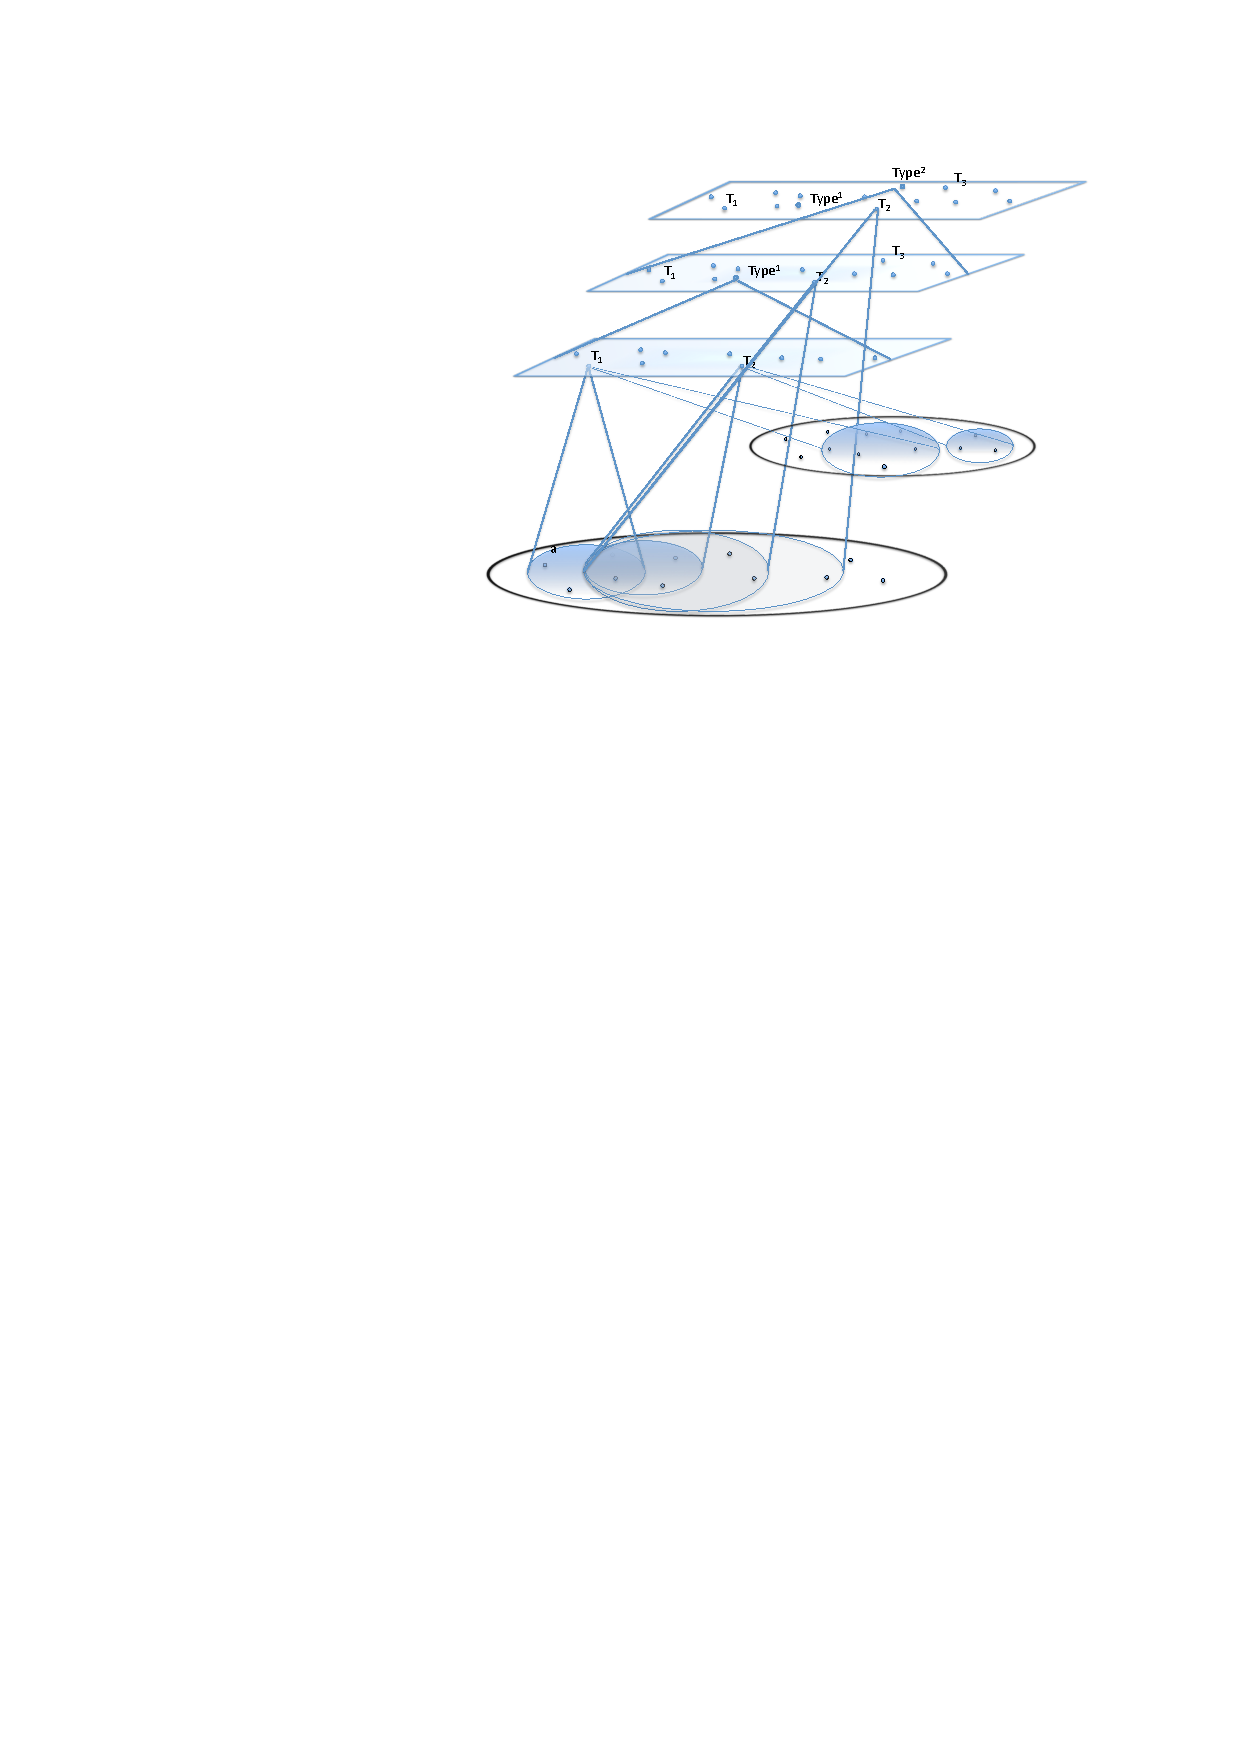
\includegraphics[width=\textwidth]{intensionalmodal}
\begin{adjustbox}{max width=\textwidth}
\begin{tikzpicture}[
  type/.style={circle, inner sep=0pt, minimum size=6pt, ball color=BTypeCol},
  firsttype/.style={circle, inner sep=0pt, minimum size=6pt, ball color=FirstTypeCol},
  secondtype/.style={circle, inner sep=0pt, minimum size=6pt, ball color=SecondTypeCol},
  objects/.style={circle, inner sep=0pt, minimum size=6pt, ball color=ObjectCol},
  modalobjects/.style={circle, inner sep=0pt, minimum size=6pt, ball color=ModalCol}
  ]

  % basic types:
  \begin{scope}[
    % every node/.append style={yslant=0,xslant=1.75},
    yslant=0,xslant=1.75
    ]
    \filldraw [fill=BTypeCol, draw=BorderCol, thick, fill opacity=0.5] (0,0) rectangle (8,2);

    \foreach \x/\y in {0.5/1.3, 1.4/1.6, 1.8/1.3, 1.9/0.5, 3.3/1.8, 2.6/1.5, 4.4/0.9, 4.7/1, 5.5/0.3, 5.6/1.1, 5.5/1.7, 6.4/1.2, 6.7/1.6} {
      \node [type] at (\x,\y) {};
    }

    \node [coordinate] (btypeleft) at (0,1) {};
    \node [coordinate] (btyperight) at (8,1) {};

    \node [type, label=above:$T_1$] (t1) at (1.3,0.6) {};
    \node [type, label=above:$T_2$] (t2) at (4.5,0.5) {};
  \end{scope}    


  % objects:
  \begin{scope}[
    % every node/.append style={yslant=0,xslant=1.75},
    %yslant=0,xslant=1.75,
    yshift=-100
    ]
    \filldraw [fill=ObjectCol, opacity=0.4, draw=BorderCol, ultra thick] (5,0) ellipse (6 and 1);

    \foreach \a/\b in {5.5/0.7, 6.4/0.2, 6.7/0.6, 7/0, 7.5/0.35, 8/-0.3, 8.1/0.2, 8.7/0, 9/0.2, 10/0.1} {
      \node [objects] at (\a,\b) {};
    }
    % for T1 from BType:
    \node [objects] (o1) at (0.3,-0.1) {}; 
    \node [objects] (o2) at (1,0.35) {}; 
    \node [objects] (o3) at (1.6,-0.2) {};
    \node [ellipse, fit=(o1) (o2) (o3), yscale=0.7, draw=BTypeCol, thick, fill=BTypeCol, fill opacity=0.3] (fitA) {};
    \draw [BTypeCol, thick] (t1) -- (fitA.east);
    \draw [BTypeCol, thick] (t1) -- (fitA.west);

    % for T2 from BType:
    \node [objects] (o4) at (2.6,-0.5) {};
    \node [objects] (o5) at (3.1,-0.5) {};
    \node [objects] (o6) at (3.3,-0.1) {};
    \node [ellipse, fit=(o3) (o4) (o5) (o6), yscale=0.7, xscale=0.7, draw=BTypeCol, thick, fill=BTypeCol, fill opacity=0.2] (fitB) {};
    \draw [BTypeCol, thick] (t2) -- (fitB.east);
    \draw [BTypeCol, thick] (t2) -- (fitB.west);

    % for T2 from Type1:
    \node [objects] (o7) at (4,0.4) {};
    \node [objects] (o8) at (4.4,0) {}; 
    \node [objects] (o9) at (4.7,0.1) {};
    \node [ellipse, fit=(o3) (o4) (o5) (o6) (o7) (o8) (o9), yscale=0.9, xscale=0.8, draw=FirstTypeCol, thick, fill=FirstTypeCol, fill opacity=0.2] (fitC) {};

    % for T2 from Type2:
    \node [objects] (o10) at (5.5,-0.3) {};
    \node [objects] (o11) at (5.6,-0.1) {};
    \node [ellipse, fit=(o3) (o4) (o5) (o6) (o7) (o8) (o9) (o10) (o11), yscale=0.95, xscale=0.85, draw=SecondTypeCol, thick, fill=SecondTypeCol, fill opacity=0.2] (fitD) {};
  \end{scope}


  % modal types:
  \begin{scope}[
    % every node/.append style={yslant=0,xslant=1.75},
    %yslant=0,xslant=1.75,
    yshift=-35, 
    xshift=220
    ]
    \filldraw [fill=ObjectCol, opacity=0.4, draw=BorderCol, ultra thick] (3.5,0) ellipse (4 and 0.75);

    \foreach \a/\b in {0.3/-0.1, 1.5/-0.3, 3.9/0.2, 7/0} {
      \node [objects] at (\a,\b) {};
    }
    \node [objects] at (0.7,0) {};
    \node [objects] (i1) at (5.7,-0.2) {};
    \node [objects] (i2) at (6.1,0.3) {};
    \node [objects] (i3) at (5,0) {};
    \node [ellipse, fit=(i1) (i2) (i3), yscale=0.7, draw=BTypeCol,
    thick, fill=BTypeCol, fill opacity=0.2] (fitAA) {};
\draw [BTypeCol, thick] (t2) -- (fitAA.north);
    \draw [BTypeCol, thick] (t2) -- (fitAA.south west);

    \node [objects] (i4) at (1.6,0.1) {};
    \node [objects] (i5) at (2,0.2) {};
    \node [objects] (i6) at (2.5,-0.3) {};
    \node [objects] (i7) at (2.7,0.35) {};
    \node [ellipse, fit=(i4) (i5) (i6) (i7), yscale=0.7, xscale=1.1,
    draw=BTypeCol, thick, fill=BTypeCol, fill opacity=0.2] (fitBB) {};
    \draw [BTypeCol, thick] (t1) -- (fitBB.north);
    \draw [BTypeCol, thick] (t1) -- (fitBB.south west);
  \end{scope}


  % Type1:
  \begin{scope}[
    % every node/.append style={yslant=0,xslant=1.75},
    yslant=0,xslant=1.75,
    xshift=-100,
    yshift=80
    ]
    \filldraw [fill=FirstTypeCol, draw=BorderCol, thick, fill opacity=0.3] (0,0) rectangle (8,2);
    \node [coordinate] (firsttypeleft) at (0,1) {};
    \node [coordinate] (firsttyperight) at (8,1) {};

    \foreach \x/\y in {0.45/1.4, 1.4/1.6, 1.9/0.5, 3.3/1.8, 2.6/1.5, 4.7/1, 5.5/0.3, 5.6/1.1,  6.7/1.6} {
      \node [firsttype] at (\x,\y) {};
    }

    \node [firsttype, label=above:$T_1$] (ft1) at (1.8,1.1) {};
    \node [firsttype, label=above:$T_2$] (ft2) at (5.8,0.7) {};
    \node [firsttype, label=above:$T_3$] (ft3) at (6.4,1.2) {};
    \node [firsttype, label=above:{\textbf{Type$^1$}}] (ft) at (4,0.4) {};

    \draw [FirstTypeCol, thick] (ft) -- (btypeleft);
    \draw [FirstTypeCol, thick] (ft) -- (btyperight);
    
    \draw [FirstTypeCol, thick] (ft2) -- (fitC.east);
    \draw [FirstTypeCol, thick] (ft2) -- (fitC.west);
  \end{scope}    


  % Type2:
  \begin{scope}[
    % every node/.append style={yslant=0,xslant=1.75},
    yslant=0,xslant=1.75,
    xshift=-200,
    yshift=160
    ]
    \filldraw [fill=SecondTypeCol, draw=BorderCol, thick, fill opacity=0.1] (0,0) rectangle (8,2);
    \foreach \x/\y in {1.4/1.6, 1.9/0.5, 3.2/1.5, 4.7/1, 5.4/1.2, 5.8/0.3, 6/0.3,  6.2/1.6} {
      \node [secondtype] at (\x,\y) {};
    }

    \node [secondtype, label=above:$T_1$] (st1) at (1.2,1) {};
    \node [secondtype, label=above:$T_2$] (st2) at (4.8,0.7) {};
    \node [secondtype, label=above:$T_3$] (st3) at (6.4,1.2) {};
    \node [secondtype, label=above:{\textbf{Type$^1$}}] (st4) at
    (3.4,0.5) {};
    \node [secondtype, label=above:{\textbf{Type$^2$}}] (st) at
    (4.0,1.7) {};

    \draw [SecondTypeCol, thick] (st) -- (firsttypeleft);
    \draw [SecondTypeCol, thick] (st) -- (firsttyperight);
    
    \draw [SecondTypeCol, thick] (st2) -- (fitD.east);
    \draw [SecondTypeCol, thick] (st2) -- (fitD.west);
  \end{scope}    
\end{tikzpicture}
\end{adjustbox}

\caption{Intensional modal type system}
\label{fig:intensionalmodal}
\end{figure}

\section{Summary}


%%% Local Variables: 
%%% mode: latex
%%% TeX-master: "ttl"
%%% End: 
